\documentclass[degree=master,tocarialchapter,openany,oneside]{thuthesis}
% 选项
%   degree=[bachelor|master|doctor|postdoctor], % 必选,学位类型
%   language=[chinese|english], % 可选(默认:chinese),论文的主要语言
%   secret,                % 可选(默认:关闭),是否有密级
%   tocarialchapter,       % 可选(默认:关闭),章目录中使用黑体(这项表示同时打开下面两项)
%   tocarialchapterentry,  % 可选(默认:关闭),单独控制章标题在目录中使用黑体
%   tocarialchapterpage,   % 可选(默认:关闭),单独控制章页码在目录中使用黑体

% 所有其它可能用到的包都统一放到这里了,可以根据自己的实际添加或者删除。
%tiansongyu add somethings start
\usepackage{multirow}
\usepackage{xcolor}
\usepackage{listings}

\usepackage{latexsym}
%\usepackage{lmodern}

% end 
\usepackage{thuthesis}
\usepackage{siunitx}
\usepackage{algorithm}
\usepackage{algorithmic}
\usepackage{amsmath}
\usepackage{bm}
\usepackage{tikz}
\usepackage{amsmath}
\usetikzlibrary{shapes.geometric}
\usepackage{tabularx}
\floatname{algorithm}{算法}
\renewcommand{\algorithmicrequire}{\textbf{输入:}}
\renewcommand{\algorithmicensure}{\textbf{输出:}}
\newcolumntype{C}{>{\centering\arraybackslash}X}
% 定义所有的图片文件在 figures 子目录下
\graphicspath{{figures/}}

% 可以在这里修改配置文件中的定义。导言区可以使用中文。
% \def\myname{薛瑞尼}

\begin{document}

%%% 封面部分
\frontmatter
\thusetup{
  %******************************
  % 注意:
  %   1. 配置里面不要出现空行
  %   2. 不需要的配置信息可以删除
  %******************************
  %
  %=====
  % 秘级
  %=====
  secretlevel={秘密},
  secretyear={10},
  %
  %=========
  % 中文信息
  %=========
  ctitle={抗逆向分析 PE 文件保护系统研究与实现},
  cdegree={工程硕士},
  cdepartment={计算机科学与技术学院},
  cmajor={计算机技术},
  cauthor={田淞煜},
  csupervisor={李鹏},
  cassosupervisor={}, % 副指导老师
  ccosupervisor={}, % 联合指导老师
  % 日期自动使用当前时间,若需指定按如下方式修改:
  cdate={2021年4月},
  %
  % 博士后专有部分
  catalognumber     = {TP666},  % 可以留空
  udc               = {UDC},  % 可以留空
  id                = {编号},  % 可以留空: id={},
  cfirstdiscipline  = {计算机科学与技术},  % 流动站(一级学科)名称
  cseconddiscipline = {系统结构},  % 专 业(二级学科)名称
  postdoctordate    = {2009 年 7 月——2011 年 7 月},  % 工作完成日期
  postdocstartdate  = {2009 年 7 月 1 日},  % 研究工作起始时间
  postdocenddate    = {2011 年 7 月 1 日},  % 研究工作期满时间
  %
  %=========
  % 英文信息
  %=========
  etitle={Research and implementation of PE file protection system for antistress analysis},
  % 这块比较复杂,需要分情况讨论:
  % 1. 学术型硕士
  %    edegree:必须为Master of Arts或Master of Science(注意大小写)
  %             “哲学、文学、历史学、法学、教育学、艺术学门类,公共管理学科
  %              填写Master of Arts,其它填写Master of Science”
  %    emajor:“获得一级学科授权的学科填写一级学科名称,其它填写二级学科名称”
  % 2. 专业型硕士
  %    edegree:“填写专业学位英文名称全称”
  %    emajor:“工程硕士填写工程领域,其它专业学位不填写此项”
  % 3. 学术型博士
  %    edegree:Doctor of Philosophy(注意大小写)
  %    emajor:“获得一级学科授权的学科填写一级学科名称,其它填写二级学科名称”
  % 4. 专业型博士
  %    edegree:“填写专业学位英文名称全称”
  %    emajor:不填写此项
  edegree={Master of Engineering},
  emajor={Computer Science and Technology},
  eauthor={Tian Songyu},
  esupervisor={Professor Zheng Weimin},
  eassosupervisor={Chen Wenguang},
  % 日期自动生成,若需指定按如下方式修改:
  % edate={December, 2005}
  %
  % 关键词用“英文逗号”分割
  ckeywords={虚拟软件加壳,代码混淆,PE文件保护,逆向工程,软件保护},
  ekeywords={Virtual software packing, code obfuscation, PE file protection, reverse engineering, software protection}
}

% 定义中英文摘要和关键字
\begin{cabstract}
%在软件行业快速发展的同时,软件逆向工程技术和二进制分析技术也在 快速发展和进步,使得逆向软件分析者对软件的逆向能力和分析效率大大提 高,给软件安全保护工作带来极大挑战。

为应对逆向分析给 Windows 软件带来的安全威胁,本文提出并实现一个针对 Windows 可执行程序的安全保护系统,该系统对可执行程序逆向中的静态分析和动态分析过程进行保护,有效提高逆向分析者的分析难度。采取的主要保护措施有:一、加壳,在已有虚拟机加壳技术的基础上进行改进,提出多样化Handler的保护机制;二、代码混淆、通过对软件进行混淆处理,改变程序的运行时的函数块的结构并增加指令的复杂度,以此来增加逆向分析难度。本文以增强 PE 文件的抗逆向能力为目的,对 Windows 平台下的 PE 文件 的二进制混淆技术和虚拟机加壳技术进行研究,主要工作包括:

首先,分析Windows下PE文件的加壳技术和二进制保护技术的研究现状,对PE文件抗逆向分析的常见方法进行总结,简单阐述PE文件加壳原理和市面流行壳的类型分析。

其次,对基于虚拟机的多样化Handler加壳保护方式进行详细阐述,对建立的数据结构、调用约定和框架都从源码的层面上进行详细解释,通过对比普通Handler实现和多样化Handler实现的优缺点,最终证明多样化Handler具有更强的抗逆向性能,进而证明所提出的加壳方法的有效性。

再次,提出建立索引的方式对函数间基本块进行交换的静态保护算法,对算法的基本思想进行简要阐述,通过对常用的反调试技术进行分析,发现常用反调试技术的局限性,在其基础上进行优化改进,在最后设计并实现一个二进制混淆器。

最后,对以上提出的加壳方式进行实验验证,通过与流行加壳软件对比压缩率、运行时间额外开销、静态和动态指令执行率等参数,间接证明提出的保护方式是有效可性的,最终实验结果得出提出的保护方式在隐蔽性、运行时间开销和占用空间等方面具有一定优势。



\end{cabstract}

% 如果习惯关键字跟在摘要文字后面,可以用直接命令来设置,如下:
% \ckeywords{\TeX, \LaTeX, CJK, 模板, 论文}

\begin{eabstract}
%With the rapid development of the software industry, software reverse engineering technology and binary analysis technology are also developing and progressing rapidly, which greatly improves the reverse-software analysts' ability and analysis efficiency of software, and brings great challenges to software security protection. 

In order to deal with the security threats brought by reverse analysis to Windows software, this paper proposes and implements a security protection system for Windows executable programs. The system protects the static analysis and dynamic analysis process in the reverse analysis of executable programs and effectively improves reverse analysis. The difficulty of the analysis. The main protection measures adopted are: 1. Packing, improving on the basis of existing virtual machine packing technology, and proposing a protection mechanism of diversified Handler; 2. Code obfuscation, changing the operation of the program by obfuscating the software The structure of the function block at the time and increase the complexity of the instruction, so as to increase the difficulty of reverse analysis. This paper aims at enhancing the anti-reverse ability of PE files, and researches the binary obfuscation technology and virtual machine packing technology of PE files under the Windows platform. The main work includes:

First, analyze the research status of PE file packer technology and binary protection technology under Windows, summarize the common methods of PE file anti-reverse analysis, briefly explain the PE file packer principle and the type analysis of popular shells in the market.

Secondly, the virtual machine-based diversified Handler shelling protection method is elaborated, and the established data structure, calling convention and framework are explained in detail from the source code level, and the advantages of common Handler implementation and diversified Handler implementation are compared. The shortcomings finally prove that the diversified Handler has stronger anti-reverse performance, and then prove the effectiveness of the proposed packing method.

Thirdly, a static protection algorithm for exchanging basic blocks between functions is proposed by establishing an index, and the basic idea of ​​the algorithm is briefly explained. Through the analysis of the commonly used anti-debugging techniques, the limitations of the commonly used anti-debugging techniques are found. Optimize and improve on the above, and finally design and implement a binary obfuscator.

Finally, the experimental verification of the above-mentioned packing method is carried out. By comparing the compression rate, runtime overhead, static and dynamic instruction execution rate and other parameters with popular packing software, it indirectly proves that the proposed protection method is effective and feasible. The experimental results show that the proposed protection method has certain advantages in terms of concealment, running time overhead and space occupation.

\end{eabstract}

% \ekeywords{\TeX, \LaTeX, CJK, template, thesis}

% 如果使用授权说明扫描页,将可选参数中指定为扫描得到的 PDF 文件名,例如:

\includepdf[pages={1,2,3,4}]{data/cover-ann-abs.pdf}
\makecover

\mainmatter
%% 目录
\tableofcontents

%% 符号对照表
%\begin{denotation}[3cm]
\item[HPC] 高性能计算 (High Performance Computing)
\item[cluster] 集群
\item[Itanium] 安腾
\item[SMP] 对称多处理
\item[API] 应用程序编程接口
\item[PI] 聚酰亚胺
\item[MPI] 聚酰亚胺模型化合物,N-苯基邻苯酰亚胺
\item[PBI] 聚苯并咪唑
\item[MPBI] 聚苯并咪唑模型化合物,N-苯基苯并咪唑
\item[PY] 聚吡咙
\item[PMDA-BDA]	均苯四酸二酐与联苯四胺合成的聚吡咙薄膜
\item[$\Delta G$] 活化自由能 (Activation Free Energy)
\item[$\chi$] 传输系数 (Transmission Coefficient)
\item[$E$] 能量
\item[$m$] 质量
\item[$c$] 光速
\item[$P$] 概率
\item[$T$] 时间
\item[$v$] 速度
\item[劝学] 君子曰:学不可以已。青,取之于蓝,而青于蓝;冰,水为之,而寒于水。木
  直中绳。輮以为轮,其曲中规。虽有槁暴,不复挺者,輮使之然也。故木受绳则直,金就
  砺则利,君子博学而日参省乎己,则知明而行无过矣。吾尝终日而思矣,不如须臾之所学
  也;吾尝跂而望矣,不如登高之博见也。登高而招,臂非加长也,而见者远;顺风而呼,
  声非加疾也,而闻者彰。假舆马者,非利足也,而致千里;假舟楫者,非能水也,而绝江
  河,君子生非异也,善假于物也。积土成山,风雨兴焉;积水成渊,蛟龙生焉;积善成德,
  而神明自得,圣心备焉。故不积跬步,无以至千里;不积小流,无以成江海。骐骥一跃,
  不能十步;驽马十驾,功在不舍。锲而舍之,朽木不折;锲而不舍,金石可镂。蚓无爪牙
  之利,筋骨之强,上食埃土,下饮黄泉,用心一也。蟹六跪而二螯,非蛇鳝之穴无可寄托
  者,用心躁也。—— 荀况
\end{denotation}



% % 也可以使用 nomencl 宏包:

% \printnomenclature[3cm]

% \nomenclature{HPC}{高性能计算 (High Performance Computing)}
% \nomenclature{cluster}{集群}
% \nomenclature{Itanium}{安腾}
% \nomenclature{SMP}{对称多处理}
% \nomenclature{API}{应用程序编程接口}
% \nomenclature{PI}{聚酰亚胺}
% \nomenclature{MPI}{聚酰亚胺模型化合物,N-苯基邻苯酰亚胺}
% \nomenclature{PBI}{聚苯并咪唑}
% \nomenclature{MPBI}{聚苯并咪唑模型化合物,N-苯基苯并咪唑}
% \nomenclature{PY}{聚吡咙}
% \nomenclature{PMDA-BDA}{均苯四酸二酐与联苯四胺合成的聚吡咙薄膜}
% \nomenclature{$\Delta G$}{活化自由能 (Activation Free Energy)}
% \nomenclature{$\chi$}{传输系数 (Transmission Coefficient)}
% \nomenclature{$E$}{能量}
% \nomenclature{$m$}{质量}
% \nomenclature{$c$}{光速}
% \nomenclature{$P$}{概率}
% \nomenclature{$T$}{时间}
% \nomenclature{$v$}{速度}



%%% 正文部分
\backmatter
\chapter{绪论}
\label{cha:intro}

\section{课题研究的目的和意义}
自第一台计算机出现以来,计算机软件安全成为计算机工程师不得花费心力思考的问题。在第一个蠕虫病毒出现之后,计算机的软件信息安全受到严重威胁。普通用户的计算机受到各种病毒和木马的威胁,其中包括大部分是通过网络传输到个人计算机中,通过修改程序的二进制代码,改变程序的执行流程,有的甚至被植入Shellcode代码,从而执行破坏或者窃取信息的代码,这是用户面临的软件程序的安全问题。

在当今互联网世界中,软件开发者的版权保护受到越来越多的关注,在二进制的层面上保护软件已经是很多软件生产公司最关注的问题之一,就算是Microsoft公司生产的Windows操作系统系列产品都会被技术水平较高的黑客破解\cite{芦天亮2020计算机病毒中的密码算法应用及防御方法综述},可见软件保护在当今互联网时代的难度之高,但是软件保护的意义不能小觑,很多商业软件依然给软件提供了各种注册方式,试图阻碍破解者获取软件正确序列号和逆向分析软件,其中包括通过网络验证、非对称加密RSA算法、机器注册码等方式。

类比于自然界植物用壳保护种子,计算机软件壳也是用来保护软件中的内容不被破解者非法修改。加壳软件在被保护软件中加入一段代码,并把原程序中代码执行区域中的代码加密、压缩,在程序正常运行时,被添加的代码会优先运行,为程序提供运行环境,包括整理堆栈、初始化CPU寄存器值等指令,最后对代码执行区域中的代码进行解密,转换为原代码后,最后将程序的执行权限交付给原程序。

软件盗版和篡改是世界面临的众所周知的威胁。已经进行了很多尝试来保护软件免受逆向工程和篡改。似乎软件开发人员和破解者之间正在进行一场战争,双方都希望随着时间的流逝相互竞争。审查了一些丰富的软件保护技术\cite{王欢2020构建高效},包括多块哈希方案,基于硬件的解决方案,校验和,混淆,防护,软件老化,加密技术和水印。所有这些技术都发挥了自己的作用,以保护软件免受恶意攻击。

软件保护在游戏行业也显得颇为重要,国内游戏软件两巨头腾讯和网易投入大量的人力资源对游戏软件加入反外挂机制,由于大部分网游都是运行在客户端,破解者可以通过分析二进制代码,使用ODDbg、IDA和WinDbg等反汇编工具对游戏进行动态或静态的反汇编\cite{徐君锋2017Android},技术较为程序的破解者通过分析汇编代码,是可以对整个游戏的流程进行细致分析,从而找出游戏中各种人物属性、技能、天赋在内存中的存放位置,最后可以使用C语言,对游戏进行远程内存注入,实现内存区域的控制,最后实现一个任意用户可用的游戏性外挂,这对当今依靠会员充值等方式盈利的公司是一个很大的打击,破解者甚至在分析游戏汇编代码后,可以构造网络游戏的网络包,直接对服务器发出伪造好的数据包,数据包中可能存放着购入金钱代码,直接对游戏进行充值,更有不法份子对这种修改软件进行售卖\cite{简容2019一种多层次的自动化通用},对游戏公司产生非常大的利益损失。

程序二进制混淆是软件开发人员和密码学专家长期以来一直感兴趣的话题。此处动机非常简单:找到一种方法,使我们可以为人们提供可以运行的程序,而无需他们弄清楚了程序是如何工作的,最后一部分必定会涉及很多内容\cite{钟林辉2020软件演化历史的逆向工程生成方法研究}。原则上,它包括从所使用的特定秘密算法的性质到可能会使用硬编码加密程序中的秘密信息等方面。

%对于一个简单的示例,请考虑一下例程:

%\begin{lstlisting}[language=C]
%// 检查密码,如果正确则打印出绝密信息
%SuperSecretPasswordProtectedStuff(string passwd) {
%if (password == “0x123”) {
%  print(“恭喜. 下面是一些重要的私人信息: ….\n”);
% } 
%else {
%  print(“密码错误.\n”);
% }
%}
%\end{lstlisting}

大多数程序都非常易于阅读,攻击者可能只是查看此程序即可恢复序列号密码\cite{徐君锋2017Android}。程序混淆的想法是,如果能够以某种方式阻止人们这样做,同时让他们拥有并在自己的计算机上运行的程序,那许多需要保护的软件都可以使用这种方式保护起来\cite{夏学云2019软件逆向工程技术分析}。

在现实世界的软件系统中,“混淆”通常是指一些临时技术的集合,这些技术将一些设计巧妙的程序变成许多GOTO代码组合,有时重要的常量会被切碎并分布在代码周围\cite{2020Malware}。该代码的某些部分甚至可以被加密,尽管是暂时的,因为解密密钥必须随程序一起提供才能真正运行\cite{2019Transforming}。

%^恶意软件作者都喜欢下图\ref{cha1:sub1:chunkcode}这种混淆。

%\begin{figure}[H]
%	\centering
%	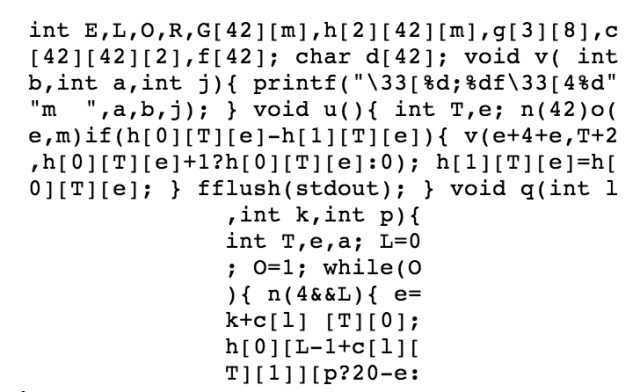
\includegraphics[width=0.7\textwidth]{chunkcode.png}\\
%	\caption{2013年C语言混淆大赛的获胜作品之一}
%	\label{cha1:sub1:chunkcode}
%\end{figure}
%尽管这些技术不错,但它们并不是真正的“不可破解”,甚至在我们想要的真正意义上也不能防止逆向工程。

只要有足够时间、精力和工具\cite{2018Analysis},人人都可以摆脱最常见的软件混淆技术\cite{2014A}。现有软件混淆的质量很差,是密码学家面临的问题。是否存在这样一个程序混淆加密器,用这样的混淆器来加密受保护的软件,同时要证明可保护所有需要保护的信息。如果能够做到这一点,它将拥有惊人的应用场景。股票交易者可以混淆其专有的交易算法\cite{2020Flow},然后将其发送到云端或者最终客户。产生的程序仍然可以正常工作\cite{0Black},但是客户永远不会学到“工作原理“的任何信息。在程序外看,程序就是一个黑匣子,而程序的内部将是各种混合机制和原有代码的融合\cite{2020A}。

%任何形式的复制保护都起源于密码学,Kerckhoffs原理是现在密码学中最重要的规则之一,它指出系统的安全性不应该取决于算法的秘密,而应该取决于密钥的秘密。因此,根据该方法构建的系统需要已知该机制,因为安全性仅基于排他性地基于可变密钥。许多加密方法都基于此原理。

因此,软件安全问题是普通用户和公司软件都不容忽视的问题,软件保护者需要开发出既能保证软件正常运行同时又避免被逆向者分析的软件保护程序,本文将针对软件保护程序进行相关技术的研究。


\section{国内外研究现状}
\label{cha1:sec:relatedworks}
在软件混淆加密技术领域,全球有诸多小组致力于此研究,也均在保证加密性能和运行性能下给出了出色的解决方案。
\subsection{国内研究现状}

浙江大学的高勇等人提出使用加密狗虚拟技术实现共享式工作平台,加密狗通常是USB记忆棒,改USB记忆棒连接到计算机上的端口以验证许可证\cite{秦飞2018逆向工程和}。使用USB加密狗运行的软件首先在启动后定期发送一个请求到I/O端口进行身份验证。一旦无法检索到与其的验证码,该程序就会自动终止,或者只能访问有限的功能\cite{Jeong2014Code}。加密狗尤其可以防止未授权的复制。原理本质上非常简单:没有加密狗,无法访问软件。现代硬件加密狗使用公私钥和对称机密过程,加密密钥不包含在应用程序的某个位置\cite{曾强2020Linux},而是安全地存储在Flash-ROM中,在其中它们无法被读出并仅用于加密和解密。除此之外,还有具有网络支持的加密狗,可以将其连接到网络中的任何计算机或服务器。许可证服务器应用程序正在此计算机上运行,并在网络中提供许可证。现在,受保护的应用程序将检查本地连接的加密狗或网络中的许可证服务器\cite{2019Analyzing},此外,还可以通过基于硬件,如CPU、主板和硬件驱动器等生成特殊的许可证密钥,讲软件许可证绑定到特定计算机,并将其存储在加密狗中。加密狗可以大大减少软件盗版,并且在数字版权管理中尤为有效,因为生成加密狗的非法副本非常困难。

在研究软件保护的初期,研究人员开发了一些相对有用的专业软件加密保护程序。但是,随着破解技术的发展,即使使用强大的加密算法,如Twofish,TEA,Blowfish以及CRC循环冗余校验和反调试技术的组合,坚固外壳ASProtect也可以通过使用免费的OllyDbg删除动态跟踪外壳后的反汇编代码。使用堆栈平衡原理在程序执行入口之前找到外壳,然后结合LoadPE工具的强大功能来导入表,导入地址表和重定位表。当前,VMProtect和驱动程序保护技术是保护软件的两种最重要的方法\cite{2020Call}。

国立台湾科技大学自动化与控制研究所使用AES算法对图像进行了加密试验,杨成雄教授提出了一种基于四维混沌系统的图像加密算法\cite{2017Access},以生成密钥并提高高级加密标准。通过使用现场可编程门阵列FPGA的流水线和并行计算功能来优化加密算法。首先,混沌系统用作加密算法的密钥生成器。接下来,在改进的高级加密标准中\cite{2018ORLIS},使用Spin-Sort和Cubic S-Box修改了ShiftRows和SubByres,并减少了加密次数。我们将加密算法和有线图像传输系统实现到基于ARM的SoC-FPGA。HPS软件在Linux上运行,用于控制FPGA加密算法和图像传输。


\subsection{国外研究现状}

比利时密码学家Vincent Rijmen和Joan Daemen开发了Rijndael分组密码\cite{段钢2003加密与解密}的子集,它们在AES选择过程中向NIST提交了提案\cite{2020Saturable}。Rijndael是具有不同密钥和块大小的密码家族。对于AES,NIST选择了Rijndael系列的三个成员\cite{0Compile2},每个成员的块大小为128位,但是具有三个不同的密钥长度:128、192和256位。AES已经被美国政府采用,现已在全球范围内使用\cite{2019Implementation}。它取代了1977年发布的数据加密标准DES。AES描述的算法是对称密钥算法,意味着同一密钥用于加密和解密数据。

麻省理工大学教授N. Sasirekha和M. Hemalatha提出了一种基于带Hadamard索引表准组加密和数字理论变换的有效安全代码方法\cite{2020Bacterial},以进行软件保护\cite{2020Detecting},此方法使用一种称为准组加密的新颖有效的加密技术对索引表进行加密。加密后,它与原始数据的相似性最小。准确有效地产生了复杂数字的密钥,这是逆向分析者难以识别原始数据。但是,准组加密在扩散纯文本的统计信息方面效率不高。因此,此方法使用链式Hadamard变换和数字理论变换将扩散与准群变换一起引入。实验结果基于时间成本和空间成本评估了所提出的加密方法的性能,并且观察到所提出的方法提供了重要的结果。



剑桥大学Barak等人提出了一种“不可区分性混淆程序”\cite{Kyu2020Clustering},简单可概括为如下内容:有两个程序$\mathit{C1}$和$\mathit{C2}$我们将它们描述为大小相似的电路,他们计算的功能相同,更具体地说,我们可以说它们具有完全相同的输入和输出行为,尽管它们在内部实现的方式可能非常不同,不可区分混淆的定义指出,应该对两个电路$\mathit{C1}$,$\mathit{C2}$进行混淆,以使没有有效的算法能够分辨$\mathit{Obf(C1)}$与$\mathit{Obf(C2)}$之间的差异。尽管这个想法是在多年前提出的,但实际上没有人知道如何构建这样的东西,称为那些“未解决的问题”之一。直到前年,情况仍然如此,直到IBM Research的一组作者基于多线程图的密码学新领域,提出了一种“候选构造”来构造这种混淆器\cite{2019White}。这个概念的另一个有趣的变种被称为萃取混淆$\mathit{Obf(EO)}$,这不仅意味着你不能分辨之间$\mathit{OBF(C1)}$和$\mathit{OBF(C2)}$,但是,如果你能区分这两种情况,那就可以找到一个输出值,$\mathit{C1}$和$\mathit{C2}$都将在该输入值上产生不同的输出。此外,其他工作表明$\mathit{IO}$和$\mathit{EO}$本质可以为常规程序提供必要好的混淆算法。

加利福尼亚大学Paul A. Cronce和Joseph M. Fontana等人提出一种将源代码转换为字节码来保护软件\cite{2019White}。他们的这种方式提供用于编程语言的语言规范,用于实现该语言的库,用于将该语言编译为字节码的编译器以及使用该库执行字节码的解释器\cite{2019Implementing};向软件发布者提供语言规范和说明,以及用于指导软件发布者如何从要保护的应用程序中选择代码部分以及如何准备所选代码部分和应用程序以在服务器上进行处理的说明,包括指示发布者在从应用程序中获取所选代码部分的相应位置创建数据结构;向服务器提供编译器、库、解释器和服务器应用程序,用于从发布者接收要保护的软件应用程序和准备好的代码选择部分。使用编译器将代码的选定部分编译为字节代码,将编译器生成的字节代码嵌入到应用程序中\cite{2018Code},并用解释程序调用替换数据结构,以调用代表已删除代码部分的适当字节代码模块的解释\cite{2018Method},从而使应用程序正确运行\cite{2018Securing},并在解释程序上运行经过混淆的代码部分和在应用程序中嵌入库和解释器以支持编译后的字节码的运行时解释,从而使所选段变得模糊\cite{2019Model}。




\section{本课题主要研究内容}

目前国内外的软件加密技术主要是使用硬件加密狗、高强度算法和使用字节码虚拟机等保护方式,以上方式都有各自的局限性,比如硬件保护方式虽然保护强度高,但是保护成本过高,每个程序的发型都需要适配一个USB硬件,不适合小型软件的发布,并且软件的运行过程由于需要插入USB设备,造成软件运行过于繁琐。高强度算法和字节码虚拟机等保护方式由于在运行过程中需要解码,所以存在软件运行效率急剧下降的问题。本文针对以上提出的问题,进行优化改进,保证了软件安全强度的前提下,尽可能提高软件的运行效率。

本文主要研究内容为:采用在反动态调试和反静态调试两个方面来防止未授权用户进行注册或者调试,反动态调试方面是对软件采用虚拟机加壳的方式,对软件进行打包,将大部分汇编代码转换为字节码,在运行时通过解释器翻译给操作系统,如果破解者不了解其中字节码和汇编代码的对应关系,将很难实现未授权注册行为;反静态调试是在已有的函数间基本块进行交换的静态保护算法基础上提出建立索引的方式对函数间基本块进行交换的静态保护算法,这种方式与剑桥大学研究内容的目标基本相同,都是对静态二进制代码进行混淆,加大IDA等静态反汇编工具的分析难度,建立索引的方式会在软件内部新增加一个节区,用来记录所有参与过函数块之间交换的块,在程序运行时,解释器会根据这个索引表进行软件的混淆机制恢复过程。

本文设计的虚拟机是一种解释执行系统与加利福尼亚大学提出的将源代码转换为字节码的原理相同,本文会提出一种基于虚拟机加壳的多样化Handler动态保护方法,在原有虚拟机保护的基础上,在二进制层面加大逆向者的分析难度,从而让软件得到更有效的保护。与解释执行语言中的虚拟机不同,本文设计的虚拟机是存在于每个可执行程序中的,所有被加密的软件都经过虚拟机加壳器的处理,其中的可执行硬编码都已经变成伪指令,即使破解者进入到虚拟机中跟踪虚拟机的解释器算法,由于每一套虚拟机的指令的不同,破解者将很难理解经过处理后的指令,破解者如果想正确逆向这样的软件,就必须对虚拟机的引擎进行深入的研究,通过不断的反复对比试验和猜测,最后形成伪指令和原始指令的对应关系,就像在破解一套摩尔斯电码但是不知道电码的字典一样,这样可以大大增加破解的难度和破译成本,也正是由于这种破解难度,虚拟机保护已经成为软件保护者的趋势。

\chapter{抗逆向分析的PE文件保护技术}
\label{cha:sensorsys}

\section{PE文件格式}
\label{cha2:sec:PEfile}

本课题的任务内容是对PE文件进行修改并保护\cite{2017Compiler},然后使之可以正常运行,所以对于PE文件结构的内容不容忽视,由于PE文件的修改都是基本本章节内容,所以后文将会对本节内容进行多次引用,本章将会对本课题涉及到的关于PE文件结构进行详细的研究,并分析出PE文件可以经本课题使用的空间。
\subsection{PE文件总体结构}
本课题的目的是保护Windows的可执行程序,通过改变可执行文件的数据结构,防止被破解者分析篡改,所以一定要对Windows下的可执行程序有详细的了解,本节内容将会对PE文件进行详细分析,明确每个数据结构的作用,同时对有价值的信息进行保护\cite{2017A}。

PE(Portable Executable)是一种32位和64位Windodws下的可执行文件,包括后缀名为DLL和EXE等的可执行文件。PE格式是一种数据结构,其中封装了Windows OS加载程序管理包装的可执行代码所需的信息。这包括用于链接的动态库引用\cite{2018c},API导出和导入表,资源管理数据和线程本地存储TLS数据。在NT操作系统上,PE格式用于EXE,DLL,SYS设备驱动程序和其他文件类型。所述可扩展固件接口EFI规范规定PE是在EFI环境标准的可执行格式\cite{2018VMGuards}。与PE类似的格式是ELF,它在Linux和大多数其他版本的Unix中使用。
	
PE文件的一个非常方便的方面是磁盘上的数据结构与内存中使用的数据结构相同。可以通过调用LoadLibrary函数将可执行文件加载到内存中,遇到的问题主要如何将PE文件的某些范围数据映射到内存地址空间中。因此,像IMAGE\textunderscore NT\textunderscore HEADERS结构体这样的数据结构在磁盘和内存中是相同的。透彻了解PE文件结构中的内容,可以全面认识PE文件在执行时在内存中的布局\cite{2016Design}。
重要的是要注意,PE文件不只是作为单个内存映射文件映射到内存中。取而代之的是,Windows加载程序查看PE文件并决定要映射到文件的哪些部分。这种映射是一致的,因为当映射到内存时,文件中的较高偏移量对应于较高的内存地址。磁盘文件中项目的偏移量可能与加载到内存后的偏移量有所不同。但是,PE文件中的信息都会在系统内存中出现\cite{李路鹿2020代码混淆技术研究综述},以使您能够从磁盘偏移量转换为内存偏移量,如图\ref{sec2:subsec3:pememory}所示。

\begin{figure}[htbp]
	\centering
	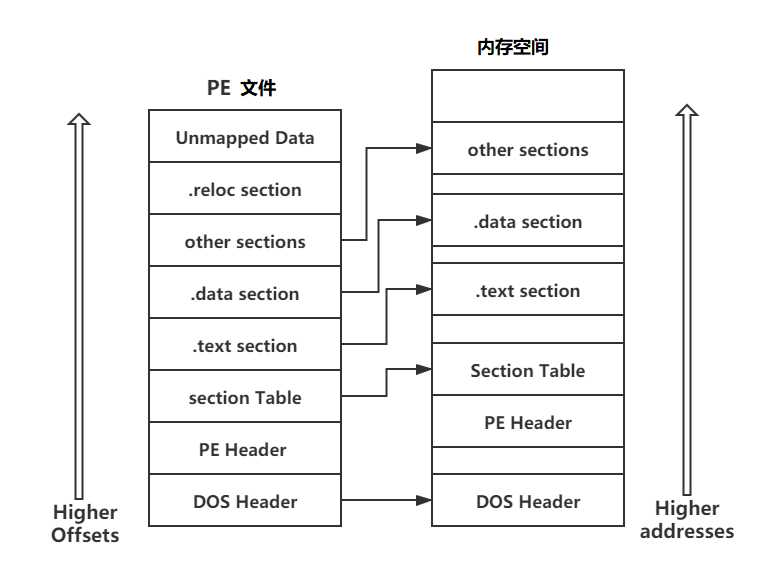
\includegraphics[width=0.9\textwidth]{pememory.png}\\
	\bicaption{PE文件运行后再内存中的节区排布情况}{After the PE file is run, then the section layout in memory}

	\label{sec2:subsec3:pememory}
\end{figure}

%PE文件的结构通常如图\ref{cha2:fig:pefile}所示:



\subsection{DOS MZ Header}

每个PE文件都以一个小型MS-DOS可执行文件开头\cite{向飞2019一种基于}。在Windows的早期,即大量的用户运行它之前,就需要此存根可执行文件\cite{吕苗苗2019基于}。在没有Windows的计算机上执行时,该程序至少可以打印出一条消息,指出要运行该可执行文件是Windows平台上的程序。

PE文件的第一个字节以传统的MS-DOS标头开始\cite{2018Enhance},称为IMAGE\textunderscore DOS\textunderscore HEADER。任何重要的仅有两个值是e\textunderscore magic和e\textunderscore lfanew字段包含PE标头的文件偏移。e\textunderscore magic字段(一个WORD)需要设置为值0x5A4D。这个值有一个\#define,名为IMAGE\textunderscore DOS\textunderscore SIGNATURE。在ASCII表示中,0x5A4D是MZ,MZ是Mark Zbikowski(MS-DOS的原始体系结构之一)的缩写。


\subsection{PE文件头}

PE Header在PE文件中的数据结构名为IMAGE\textunderscore NT\textunderscore HEADERS,IMAGE\textunderscore NT\textunderscore HEADERS结构是存储PE文件详细信息的主要位置。它的偏移量由文件开头IMAGE\textunderscore DOS\textunderscore HEADER中的e\textunderscore lfanew字段给出。IMAGE\textunderscore NT\textunderscore HEADER结构实际上有两个版本,一个用于32位可执行文件,另一个用于64位版本,两个版本的文件结构差异较小\cite{2018Construction}。微软认可的唯一正确的区分两种格式的方法是通过IMAGE\textunderscore OPTIONAL\textunderscore HEADER中的Magic字段的值。

IMAGE\textunderscore NT\textunderscore HEADER由三个字段组成,如图\ref{sec2:subsec3:image_nt_header}。

\begin{figure}[htbp]
	\centering
	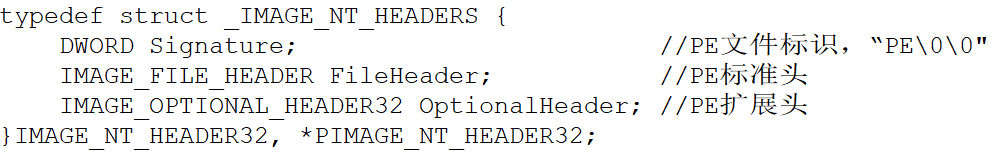
\includegraphics[width=0.9\textwidth]{image_nt_header.png}\\
	\bicaption{IMAGE\_NT\_HEADER结构定义}{IMAGE\_NT\_HEADER structure definition}
	\label{sec2:subsec3:image_nt_header}
\end{figure}

\subsection{相对虚拟地址}

在可执行文件中,有很多地方需要指定内存地址。例如,引用全局变量时需要一个绝对地址。PE文件可能在过程地址空间中的任何位置加载。虽然它们确实具有首选的加载地址,首选加载地址可能已经被使用了,这时的绝对地址就会发生改变\cite{张晓寒2020基于指令虚拟化的安卓本地代码加固方法}。因此,使用某种方式指定可执行文件加载位置的地址非常重要。

为了避免在PE文件中使用硬编码的内存地址,使用了RVA(Relative Virtual Addresses)。RVA只是相对于PE文件加载位置的内存偏移量。例如,考虑一个在地址0x400000加载的EXE文件,其代码段在地址0x401000\cite{何永瑾2020基于注册码的软件授权保护系统的设计与实现}。代码部分的RVA为:

(Target address)0x401000 - (Load address)0x400000  = (RVA)0x1000

要将RVA转换为实际地址,只需完成以下过程即可:将RVA添加到实际加载地址以找到实际的内存地址。实际的内存地址在PE术语中称为虚拟地址。定位VA的另一种方法是,使用首选加载地址的RVA通过上述方法计算得出。

\subsection{区块表}

在PE文件头IMAGE\textunderscore NT\textunderscore HEADERS结构之后的是区块表。IMAGE\textunderscore SECTION\textunderscore HEADERs结构的数组。IMAGE\textunderscore SECTION\textunderscore HEADER提供有关其关联节的信息,包括位置,长度和特征。IMAGE\textunderscore SECTION\textunderscore HEADER结构的数目由IMAGE\textunderscore NT\textunderscore HEADERS.FileHeader.NumberOfSections字段给出。


\subsection{导入表}


在PE文件中,存在名为导入表的数据结构数组,导入表给出了所有需要导入的DLL的名称,并指向一个函数指针数组。函数指针数组称为导入地址表(IAT)。每个导入的API在IAT中都有其自己的保留位置,其中,导入函数的地址由Windows加载程序编写。最后一点特别重要,加载模块后,IAT包含调用导入的API时调用的地址\cite{2018A}。

IAT的优点在于,PE文件中只有一个地方存储了导入的API地址。无论分散通过多少个源文件调用给定的API,所有调用都将通过IAT中的同一函数指针进行\cite{马雪婷2020一种共享软件保护机制的完整实现}。

下面将会通过一个实例来说明导入表的作用,有两种情况需要考虑:直接跳转和间接跳转,在直接跳转中,以执行CALL DWORD PTR [0x00405030]为例,对导入的API调用如图\ref{sec2:subsec3:direct}所示。

\begin{figure}[htbp]
	\centering
	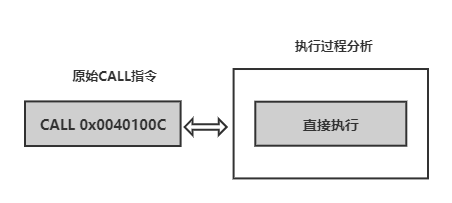
\includegraphics[width=0.6\textwidth]{direct.png}\\
	\bicaption{直接调用过程}{Direct call procedure}
	\label{sec2:subsec3:direct}
\end{figure}

CUP的EIP寄存器将会被设定为0x00405030,对导入的API使用间接跳转调用时,如图\ref{sec2:subsec3:importtable}所示。

\begin{figure}[htbp]
	\centering
	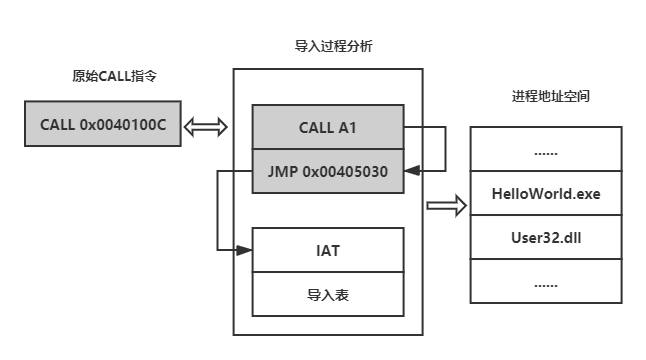
\includegraphics[width=0.9\textwidth]{importtable.png}\\
	\bicaption{使用导入表间接调用过程}{The procedure is called indirectly using the import table}
	\label{sec2:subsec3:importtable}
\end{figure}

执行的指令如下:

CALL 0x0040100C

•••

0x0040100C:

JMP       DWORD PTR [0x00405030]

在这种情况下,CALL将控制权转移到一个中继地址,中继地址中存储着API需要跳转的绝对地址0x405030。0x405030属于IAT中的一项数据。简而言之,效率较低的导入API调用使用了五个字节的附加代码,由于额外的JMP,执行时间更长。

这里使用了一个较低效率的方法来实现CALL指令,这是因为编译器无法区分导入的API调用和同一模块内的普通函数,对于编译器来说,在执行CALL指令时,将会发出如下的指令:CALL XXXXXXXX,其中XXXXXXXX是实际的代码地址,稍后将由链接器填写,这个CALL指令不是通过函数指针进行的,而是一个实际的代码地址,为了让程序正常执行,链接器需要有一段代码来代替XXXXXXXX,最简单的方式是将调用指向JMP存根\cite{2016Building}。

JMP的存根就来自导入函数的导入库,如果检查这个导入库,并且检查如导入的API名称相关的代码,会发现它是一个JMP存根。这意味着默认情况在没有任何干预的情况下,导入的API调用将使用效率较低的形式\cite{2019The}。



PE文件由许多标题和节组成,这些标题和节告诉动态链接程序如何将文件映射到内存中。可执行映像由几个不同的区域组成,每个区域需要不同的内存保护。因此,每个部分的开头必须与页面边界对齐。例如,通常.text节保存程序代码被映射为execute / readonly,而.data部分被映射为不执行/读写。但是,为避免浪费空间,不同部分在磁盘上未按页面对齐。动态链接器的部分工作是根据标题中的说明,将每个部分分别映射到内存,并为生成的区域分配正确的权限。

值得注意的一部分是导入地址表IAT,当应用程序在另一个模块中调用函数时,它用作查找表。它可以采用按序导入和按名称导入的形式。由于编译后的程序无法知道其依赖的库的存储位置,因此,每当进行API调用时,都需要进行间接跳转。当动态链接器加载模块并将它们连接在一起时,它会将实际地址写入IAT插槽,以便它们指向相应库函数的存储位置。尽管这会增加模块内调用的开销,从而导致性能下降,但它提供了一个关键的好处:需要写时复制的内存页数装入程序更改的内容最小化,从而节省了内存和磁盘I / O时间。如果编译器提前知道调用将是模块间的,则可以生成更多优化的代码,这些代码只会导致间接调用操作码。

%
在导入表中,PE文件通常不包含与位置无关的代码。相反,它们被编译为首选的基地址,并且编译器/链接器发出的所有地址都提前固定。如果PE文件无法在其首选地址加载,操作系统将重新修复它。这涉及重新计算每个绝对地址,并修改代码以使用新值。加载程序通过比较首选加载地址和实际加载地址并计算增量值来完成此操作。然后将其添加到首选地址,以提供存储位置的新地址。基地搬迁存储在列表中,并根据需要添加到现有存储位置。现在,生成的代码是该过程专用的,不再可共享,因此在这种情况下,DLL的许多节省内存的好处都丧失了。这也大大降低了模块的加载速度。因此,应尽可能避免重新基准化,Microsoft提供的DLL具有预先计算的基址,以免重叠。因此,在无基准的情况下,PE具有代码效率非常高的优点。这与使用完全与位置无关的代码和全局偏移表的ELF形成对比,后者在执行时间之间进行权衡以降低内存使用量。

在Windows NT操作系统上,PE当前支持x86,IA-32,x86-64(AMD64 / Intel 64),IA-64,ARM和ARM64 指令集体系结构。在Windows 2000之前,Windows NT因此也包括PE支持MIPS,Alpha和PowerPC ISA。由于PE在Windows CE上使用,因此它继续支持MIPS,ARM和SuperH ISA的多个变体。

以上已经对PE文件结构需要修改的地方进行了分析,本文将按照上述内容,对PE文件进行修改,实现反调试加密和虚拟机加壳功能。
\section{PE文件对抗逆向分析的常见方法}

目前市面上的大部分需要都需要软件保护措施,除去普通的方式例如序列号验证、网络注册、花指令等方式,最为普遍的就是软件加壳,软件加壳的根本目的是防止破解者对软件进行逆向分析,从而阻止他们的非法修改和逆向编译,从而保护了上述序列号验证和网络注册等方式,也可以说软件加壳的保护层面更高,如果保护得当,可以从根本上杜绝软件被非法修改。软件保护界也存在一句名言——没有不能脱的壳,所以说本课题研究的抗逆向目标也是在某种程度上加大破解的破解难度,延长他们的破解时间。软件加壳简而言之,将壳与程序通过某种方式混合在一起或进行代码变形,从而让破解者不能正确分辨软件逆向分析无用的壳代码和软件功能流程代码。软件加壳后的程序如图\ref{sec2:subsec3:aftershell}所示。

\begin{figure}[htbp]
	\centering
	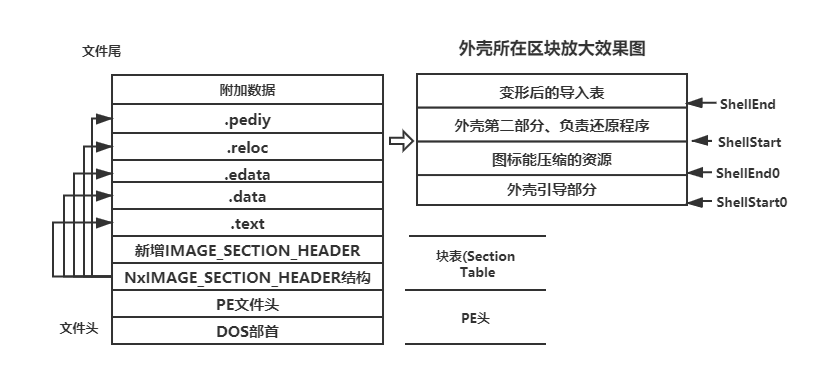
\includegraphics[width=1.0\textwidth]{aftershell.png}\\
	\bicaption{加壳后的程序的结构}{The structure of the program after shell}
	\label{sec2:subsec3:aftershell}
\end{figure}

%\subsection{加壳}
软件加壳按照方法和目的可以分为两大类,第一类是压缩壳,第二类是保护壳。保护壳是本课题的主要研究内容,这种壳的目的是加大破解者的逆向分析难度,代码会将功能代码和外壳代码混淆,可使用密钥对称加密或者非密钥加密两种方式,密钥对称加密则是在软件购买时,商家为用户提供一个私钥,用户只能通过这个私钥打开这个程序,其中的原理与普通的加密算法相仿,但是由于这种方式容易让破解者对私钥和加密代码进行分析,反而减小了破解难度,所以这种方式逐渐被淘汰,非密钥加密则是使用密码学中难以逆向分析的算法对软件进行保护。第二类的压缩壳的目的是为了减小软件的体积,但是由于软件使用了压缩算法,解密和程序运行时同时进行的,会增加程序的运行时间,压缩算法也是不断在优化当中,在时间和空间上进行取舍,这种方式基本没有保护作用,因为压缩壳并不妨碍软件破解者进行逆向分析,利用ESP栈平衡原理,很容易得到软件OEP,修复IAT表后会直接得到解压后的软件,然后再进行破解序列号的逆向分析,所以压缩壳对软件的保护作用形成虚设。

软件加壳按照保护分类可以分为两种方式,一种是本文所采用的虚拟机加壳保护,第二种是采用可执行压缩的方式。所谓可执行压缩是任何手段压缩的可执行文件,并用解压缩代码的压缩数据组合成单个可执行文件。执行此压缩的可执行文件时,解压缩代码会在执行之前从压缩的代码重新创建原始代码。在大多数情况下,压缩的保护方式是透明的,因此可以与原始文件完全相同的方式使用压缩的可执行文件。可执行压缩器通常被称为“运行时打包程序”,“软件打包程序”,“软件保护程序”,甚至是“多态打包程序”和“混淆工具”。压缩的可执行文件可以被视为自解压存档,其中压缩的可执行文件与相关的解压缩代码一起打包在可执行文件中。某些压缩的可执行文件可以解压缩以重建原始程序文件,而无需直接执行。可以用于执行此操作的两个程序是CUP386和UNP。大多数压缩的可执行文件在内存中对原始代码进行解压缩,并且大多数需要更多的内存才能运行因为它们需要存储解压缩器代码,压缩的数据和解压缩的代码。此外,某些压缩的可执行文件还具有其他要求,例如那些在执行前将解压缩的可执行文件写入文件系统的要求。

\subsection{压缩壳}
\label{cha3:sec:mutualdet}

软件程序的压缩壳软件与我们通常意义上的压缩软件如RAR不同,RAR软件压缩之后的文件格式不能被Windows内核程序加载器识别,压缩之后的文件结构已经不是EXE程序,所以不能成功运行。

压缩壳的产生时间较早,早在DOS时代,受到当时的硬件设备的限制,计算机的内存和硬盘需要严格计划使用,也受到移动存储介质的限制,软件开发者不得不想出办法来减小应用软件的占用空间,于是程序压缩技术产生了。对可执行文件进行压缩后,其内部的功能代码结构大部分发生改变,其中的汇编代码和硬编码地址已经和初始状态不能直接进行反汇编,加大了破解难度,起到了一定的反破解作用。压缩同一款产品,压缩比例越高,程序的功能代码变化越大,破解的难度也会随之提高。

压缩算法通常是使用市面上的压缩引擎,由于解压和程序的运行是同时进行的,解压会增加程序的运行时间,所以解压效率是衡量一款解压算法的重要标志,压缩的速度可以慢下来,但是解压速度需要不断的提高,如果解压速度太慢会影响用户体验。有代表性的压缩壳有ASPack、UPX和PECompact等。

ASPack是Windows下的应用程序压缩软件,市面上很多软件都使用这款压缩软件,但是由于使用用户太多,导致研究的人也多,其中的保护作用已经越来越来,现在用这款软件的目的大部分是为了减小应用软件的体积,压缩壳通常可以将可执行文件和其他依赖文件打包在一起压缩,从而减少了文件的数量,ASPack压缩后的程序是后缀为EXE的可执行文件,压缩后的程序可直接运行,并且程序的运行并不依赖ASPack这款软件,这也是与普通压缩软件差别最大的地方。

UPX(Ultimate Packer for eXecutables)是一款针对Windows的对可执行文件进行加密的文件压缩器,压缩率高达50-70$\%$,大大减小了可执行文件的磁盘占用空间,同时也减小了移动介质和网络之间的传输时间。通过UPX压缩过的程序同ASPack软件一样,不会产生功能损失会和压缩之前一样运行。其运行界面如图\ref{sec2:subsec3:upxshell}所示。

\begin{figure}[htbp]
	\centering
	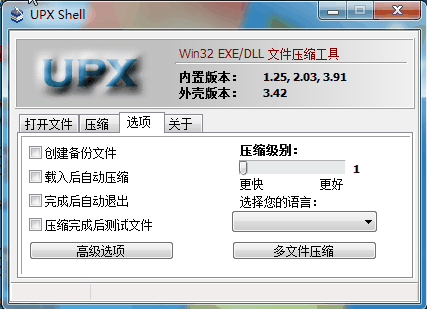
\includegraphics[width=0.7\textwidth]{upxshell.png}\\
	\bicaption{UPX加壳工具}{UPX shell tool}
	\label{sec2:subsec3:upxshell}
\end{figure}

\subsection{保护壳}
\label{cha3:sec:protectshell}
随着脱壳技术的发展,压缩壳的保护性能已经不能满足人们的需要,上述ASPack、PECompact、UPX等压缩壳软件已经形成专门针对的软件,使用压缩壳的应用程序都可以被一键脱壳,调试技术也不断提高,产生了诸多的反汇编工具ODdbg、IDA Pro等、调试工具SoftICE、OllyDbg等,随着硬件设备的性能不断提高,应用程序的占用空间和运行时间已经不是安全问题的瓶颈,防止软件被逆向、反调试技术已经成为研究的重点。于是,在加壳软件中会加入反调试的代码,比如化指令、结构异常处理机制、加密算法、代码混淆等技术,抗逆向技术在不断发展。

保护壳可以自动给应用程序添加安装包保护性外壳程序,并强制在应用程序运行之前确认安全令牌的存在和状态。保护壳还会对软件中的代码和数据进行加密,以防止进行逆向功能,使用这种保护方法,可以在不修改源代码的情况下应用软件保护。有代表性的保护壳有ASPprotect、ACProtect、Armadillo等。

ASProtect是主要面向Windows用户的软件加壳保护软件,这款软件通过RSA加密算法生成唯一KEY,通过对称加密的方式,为用户分配私钥,只有得到私钥的用户,才能在程序运行时对加密功能代码进行正确解密。内置反调试引擎,自己有一套反调试系统,在运行时会开启一个线程,检测自身是否被调试,如果被调试,则直接中断程序,给破解者的破解带来难度。其运行界面如图\ref{sec2:subsec3:asprotect}

\begin{figure}[htbp]
	\centering
	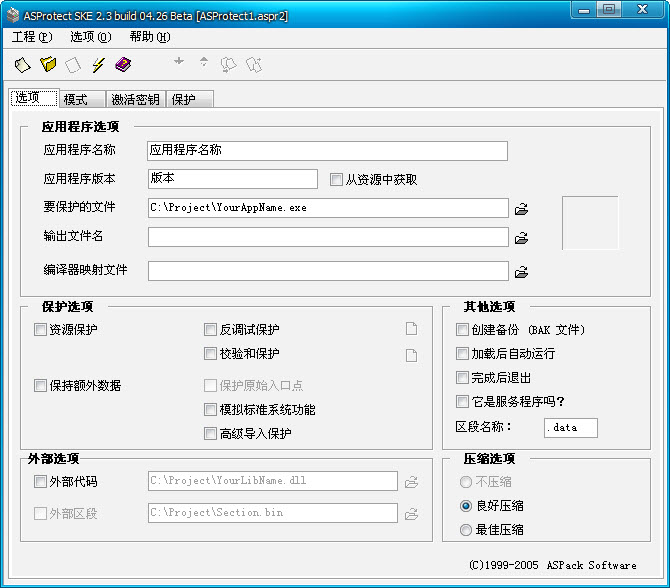
\includegraphics[width=0.8\textwidth]{asprotect.jpg}\\
	\bicaption{ASProtect加壳工具}{ASProtect packing tool}
	\label{sec2:subsec3:asprotect}
\end{figure}

\subsection{工具脱壳}

被加壳软件在运行时是需要脱壳后才会正常执行,软件脱壳就是软件加壳的逆向操作。根据脱壳方式的不同,脱壳方式分为手工脱壳和工具脱壳,工具脱壳通常只适应于流行的加壳软件,越是流行的加壳工具,研究它的人越多,拥有高技术的破解者则可以完全研究明白加壳机制后,写出自动化脱壳机,但是这种自动化脱壳机通常只针对压缩壳。

工具脱壳通常主要分为两类:专业脱壳软件和通用脱壳软件。专业脱壳软件通常只针对一种或两种加壳软件,由于是针对性的软件,脱壳成功率也相对较高。通用脱壳软件通常针对保护性能低的压缩壳,它具有通用性,可以脱掉多种不同的壳。常见的脱壳软件有UnPECompact、UnASPack、UPXShell等。

\subsection{手工脱壳}

通常的压缩壳,都有对应的自动脱壳机,但只针对于压缩壳,由于保护壳的机制太过复杂,
很难写出自动脱壳机,所有保护壳通常需要手工脱壳。

要想手工脱壳需要对PE文件以及程序加载后在内存中的数据非常了解。软件加壳技术的发展总是伴随着脱壳技术的进步,要研究脱壳技术,首先要分析壳的加载过程。壳的加载过程可以分为五个步骤,定位壳需要的所有API地址、解密函数对块(Section)的操作、重定位、EIP设置为OEP(Original Entry Point)、HOOK-API,在程序被脱壳之后,加壳进程将会把CPU的控制权还给原程序,此时原程序就会像没有加壳时的状态正常运行,原本被加密过的各种节区块都会被还原。而此时,则是脱壳程序最关键的时机,此时的程序在内存中的形态和程序没有被加壳过的形态几乎完全一致\cite{2018Method}。

手动脱壳通常分为三个步骤:一是找到程序真正入口点OEP;二是dump下内存映像文件;三是输入表的重建过程。



\subsection{壳的类型分析}

在手工脱壳之前,通常要对软件进行加壳分析,一是分析是否加了壳,二是可以分析出此程序使用了哪种壳或者本程序是用哪种语言编写。这时通常使用市面上流行的PEiD或者FileInfo等工具。PEiD的图形界面如图\ref{sec2:subsec3:peid}所示。

\begin{figure}[htbp]
	\centering
	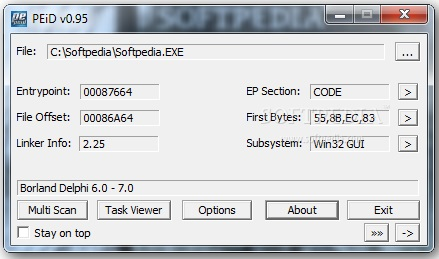
\includegraphics[width=0.8\textwidth]{peid.jpg}\\
	\bicaption{PEiD侦壳工具}{PEiD debugger}
	\label{sec2:subsec3:peid}
\end{figure}

将程序加载到PEiD中,此程序通常会给出很多有用的信息,比如壳的类型和本程序使用的编译器。此程序使用特征码做出识别判断,每种壳都有固定的特征码,只要文件搜索特征码,大部分情况下都可以识别成功,但是对于那种小众加壳或者未被公布的加密壳却无能为力,这也是本课题最终的研究目标。本软件提供了一个扩展接口USERDB.txt,用户可以自定义一些已知的特征码,通过这种方式可以识别出大部分的壳。

加壳与脱壳总是在不断博弈中,正因为PEiD是使用特征码方式识别加壳类型,加壳软件也可以伪造特征码,比如加壳软件在壳中放入多种不同类型的加壳软件特征码,这时PEiD就会失去它的作用,这种方式也被称为"PEiD欺骗”。
%%%%%%%%%%%%%%%%%%%%%%%%%%%%%%%%%%%%%%%%%
%添加一点东西,是之到下一行
\section{本章小节}
本章节对虚拟机加壳和二进制代码混淆的相关技术进行了阐述,并对PE文件结构进行了分析,对其中的DOS头、PE Header、相对虚拟地址等重要结构进行了详细阐述,并简要说明了反调试的原理,说明了在汇编语言和硬编码语言的层面上对Windows下的执行文件进行修改的相关技术,从而可以保证修改文件的正确性和可重用性。
\chapter{多样化Handler虚拟机加壳的研究与实现}

在软件反逆向工程中的虚拟机和虚拟机模拟软件是完全不同的东西,本章描述的虚拟机保护方法是类似于一种解释执行系统,它和解释型语言如Python、Lua、Ruby等有相似的地方。

%本节会对虚拟机加壳方案进行设计,并且详细叙述加密过程和解密过程,如图\ref{cha2:fig:addshell}所示
对于PE文件结构,在\ref{cha2:sec:PEfile}节有详细的分析结果,对于虚拟机加壳比较重要的位置是节表Section Table,原始PE程序的二进制硬编码通常是按照顺序排列在多个节表中的,在通过分析PE文件的DOS Header和PE Header后,可以通过里面的相关信息,计算出Section Table的起始偏移地址,得到代码区域的地址后,将此部分标记为待保护汇编的指令流的起始区域,由次区域开始到下一个.rdata节截止,对原始PE程序的二进制硬编码进行加密保护。

%\begin{figure}[h] 
%	\centering
%	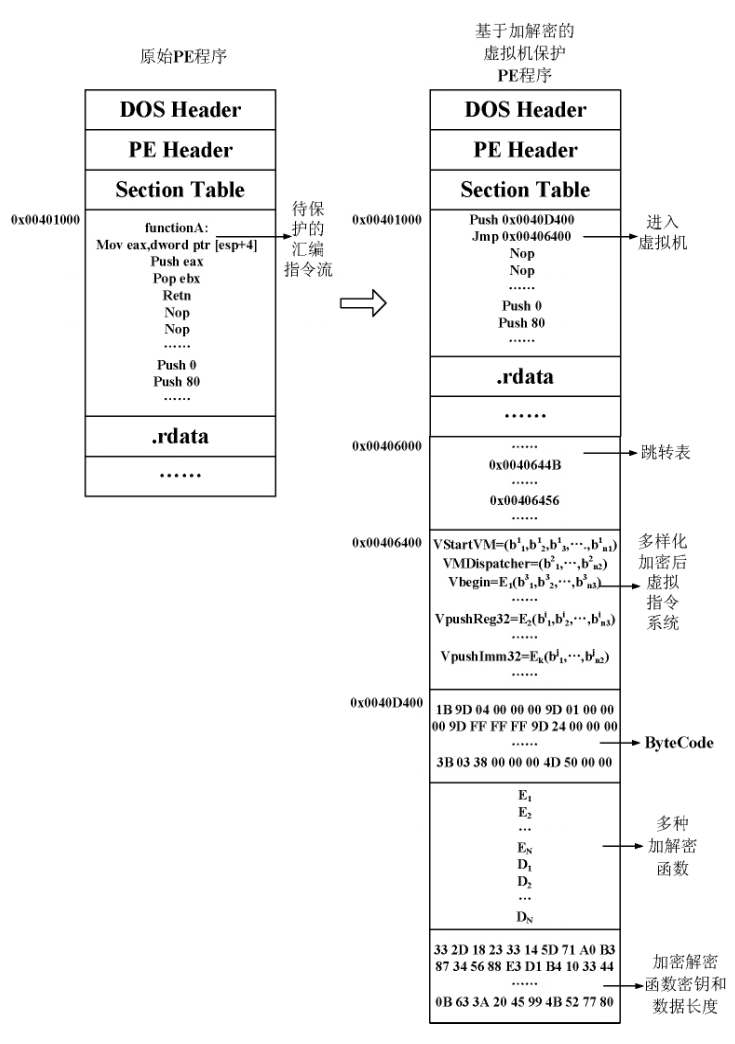
\includegraphics[height=18cm]{addshell.png}
%	\caption{虚拟机加壳过程}
%	\label{cha2:fig:addshell}
%\end{figure}


本章节将会设计一个在PE程序中的虚拟机壳,程序的OEP(Original Entry Point)程序的入口点将会被改变为虚拟机的入口点,进行虚拟机的执行区域。虚拟机将会进行一系列的初始化工作:对原有的汇编代码进行整理、提取出其中的导入表信息、建立Handler等。建立调度器dispatcher,调度器会将原本的寄存器符号统统压入栈中,把esi指向虚拟机字节码的起始地址,ebp指向当前的真实栈区域,edi指向VMContext虚拟环境结构,在执行上述过程后,虚拟机初始化环境将会加载完毕。



\section{虚拟机保护方法基本原理}


首先虚拟机保护系统会将可执行程序反汇编为CUP可以理解的X86指令流,做出一套X86指令和字节码之间的映射,再讲X86指令流的汇编代码转换为字节码,此时可执行程序已经完成了压缩阶段。最后,虚拟机保护会系统会将解释器内嵌到可执行程序中,使得被保护的代码在程序执行时可以被正确翻译后执行,整个流程类似于Java的虚拟机。

具体保护步骤如下:

Step1 将带保护程序使用反汇编引擎转换为汇编指令;

Step2 将汇编指令转换为一对一的字节码;

Step3 建立Handler表和跳转表;

Step4 将上述三个步骤产生的文件打包为可执行文件,使用虚拟环境结构VMContext存储寄存器中的值,将字节码、虚拟环境结、Handlers、Dispather打包为一个新节,并添加到可执行程序中,虚拟机代码保护机制的流程如图\ref{codeprotect}所示 。
\begin{figure}[htbp]
	\centering
	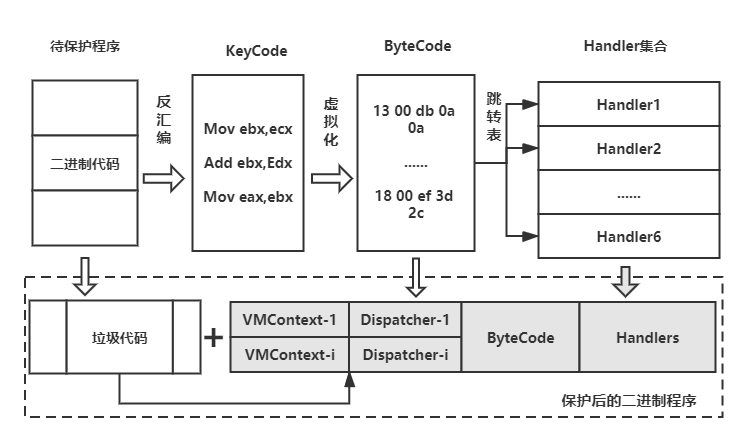
\includegraphics[width=14cm]{codeprotect.png}
	\bicaption{虚拟机代码保护机制}{Virtual machine code protection mechanism}
	\label{codeprotect}
\end{figure}

\subsection{相关反汇编工具}

反汇编器是把高级语言写成的程序翻译成汇编语言的工具,反汇编程序的目标是高级语言如C/C++、VB,而不是汇编语言,它通常输出为了便于阅读而不是适合汇编程序输入而设置的格式,反汇编器会给阅读反汇编代码者提供大量的可参考数据\cite{张泉2018Win32}。

本课题采用的是OllyDbg引擎提供的开源反汇编器,在进行反汇编过程中,它可以自动跟踪寄存器、识别函数、API调用,给阅读者带来很大的方便,由于其易用性和可用性,此软件在分析恶意代码时也很有用\cite{乐德广2018一种抵御逆向工程的安卓应用混淆技术研究}。

\subsection{X86指令}

按照x86体系结构,按照功能分为流指令、普通指令、栈指令、和不可模拟指令4类\cite{曹宏盛2019一种用于}。

流指令是指跳转指令、函数调用指令、返回指令等改变文件执行流程的指令。

普通指令指add、sub、mov等加减运算和数据传输指令。

栈指令指压栈指令弹出栈指令等操作栈空间的指令。

不可模拟指令指无法被模拟的指令,这类指令通常硬件相关,比如int3、in、out等指令。

指令分类如表\ref{registers}所示。

\begin{table}[htbp]
	\bicaption{X86汇编指令分类}{X86 assembly instruction classification}
	\label{registers}
	\begin{tabular}{l|l|l|l|l|l}
		\hline
		\multicolumn{2}{c|}{无操作数指令} & 单操作数指令 & \multicolumn{2}{l|}{双操作数指令} & 多操作数指令 \\ \hline
		AAA          & STC           & CALL   & ADC         & XADD          & IMUL   \\ \hline
		AAD          & STD           & JMP    & ADD         & XCHG          & SHLD   \\ \hline
		AAM          & STI           & JCC    & AND         & CMP           & SHRD   \\ \hline
		AAS          & INSB          & LOOP   & MOV         & CMPS          & -      \\ \hline
		CBW          & INSW          & LOOPE  & OR          & LEA           & -      \\ \hline
		CDQ          & INSD          & LOOPNE & RCL         & MOVSX         & -      \\ \hline
		CLD          & LAHF          & INC    & RCR         & MOVZX         & -      \\ \hline
		CLI          & LODSB         & DEC    & ROL         & -             & -      \\ \hline
	\end{tabular}
	\centering

\end{table}

基于虚拟机Handler动态加密的情况大致如图\ref{virtual}所示。其中VStartVM部分初始化虚拟机,VMDispatcher调度每一个Handler。在程序运行时,字节码就是操作系统需要识别的二进制代码,VMregisters就是操作系统的调度器,不同的Handler对应不同的汇编代码,相对应的就是机器码。

\begin{figure}[htbp]
	 
	\centering
	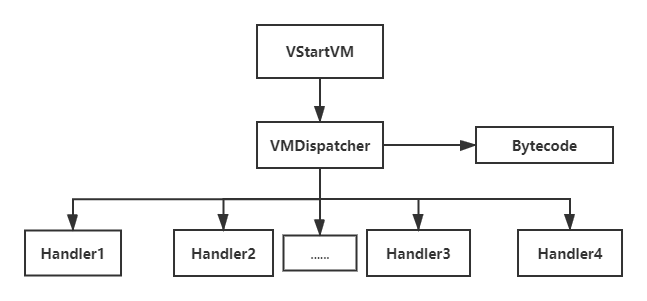
\includegraphics[height=6cm]{virtual.png}
	\bicaption{虚拟机执行时的情况}{When the virtual machine executes}
	\label{virtual}
\end{figure}



\section{调用约定和框架}

\subsection{虚拟环境}
\label{cha3:sec:virtualcontext}
解释器在执行时识别的是字节码,所以需要使用一个结构来保存CPU中寄存器的值,其结构设计具体如图\ref{context}所示\cite{胡浔惠2019一种应用随机森林的代码混淆路径分支技术}。

\begin{figure}[htbp]
	
	\centering
	
	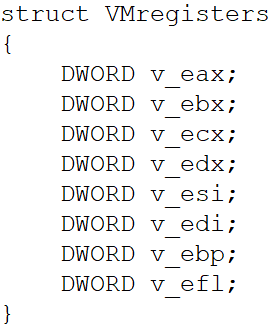
\includegraphics[height=5cm]{symbol.png}
	\bicaption{虚拟环境结构}{Virtual environment structure}
	\label{context}
\end{figure}

使用VMregisters结构体来存储eax,ebx等重要的寄存器,需要注意的是,这个结构体中不需要存放esp这个寄存器的,esp一直指向栈顶,而程序的执行本身需要栈空间的,esp寄存器的值就是ebp寄存器的值。

\subsection{调度器}

MbeginVM将原程序的环境中大部分寄存器的值压栈之后会建立一个VMDispatcher标签,Handler会循环执行这部分代码,如图\ref{begin}所示的代码MbeginVM部分也称为调度器。

\begin{figure}[htbp]
	\centering
	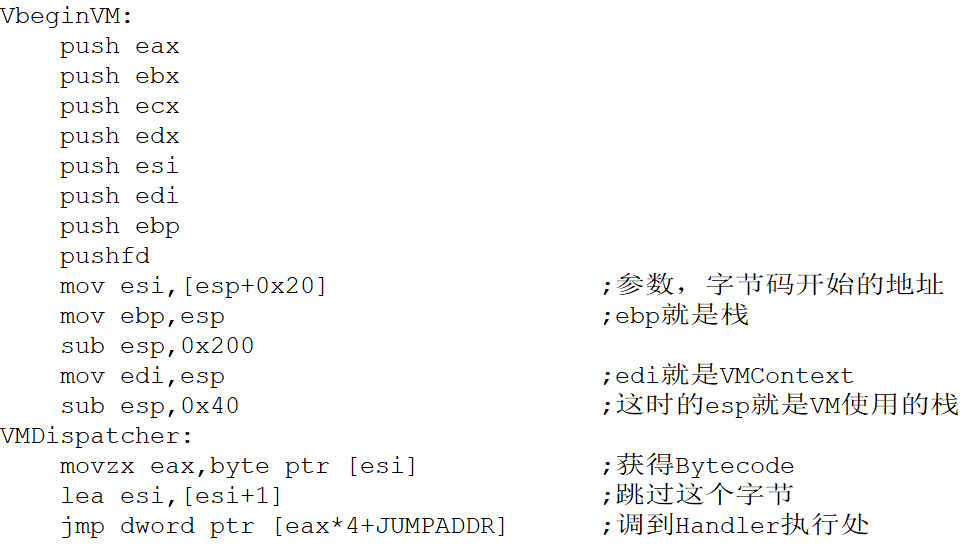
\includegraphics[height=8cm]{begin.png}
	\bicaption{Handler核心执行代码}{The Handler core executes the code}
	\label{begin}
\end{figure}


首先,调度器会将所有的CPU寄存器压栈,esi是设计的字节码的开始地址,ebg是原程序的栈空间,edi是虚拟环境结构,esp减去50h(不固定)就是虚拟机使用的栈空间地址。将虚拟机的虚拟环境结构和栈空间都放在了当前栈的300h处。

由于栈空间是变化的,这块区域可能在执行时被使用栈空间的语句覆盖,所以要设定一个机制保护本区域,当虚拟机在执行有关栈空间的指令时,需要有代码检查使用的空间是否覆盖到这块存放的数据,如果覆盖,则将这块结构向下移动。从“movze eax,byte ptr[esi]”指令开始读字节码。读取一个字节,就到跳转表中找到相应的Handler并执行相关语句。

这里会产生三个寄存器和某些值一直是对应关系,edi始终和虚拟环境结构的值相同,esi是当前字节码的地址,ebp一直是真实栈的地址。这三个对应关系在整个虚拟机执行过程中是一直成立的。通常情况下,这三个寄存器只能用作上述三个功能,不能使用做其他用途,如果必须使用则需要使用pushad来保护起所有的寄存器,在使用后需要使用popad恢复所有寄存器的值。


\section{多样化Handler设计}

本文所说Handler与Windows中的句柄Handler不同,本文的Handler指把某一段代码表示的功能给包装起来,形成可重复使用的功能结构块,它通常是被虚拟机保护中的调度器使用。Handler结构是虚拟机保护系统的核心部分,通常也是逆向攻击者的重点攻击对象,Handler结构中存放着字节码和汇编代码之间的转化过程,虽然可能这个转化过程不是通过一个Handler实现的,可能是由多个有着不同功能的Handler共同实现的,但是保护Handler等于保护了核心的翻译模块。所以,对Handler进行保护显得尤为重要,本节将会描述一种通过设计多样化的Handler使得逆向攻击者难以逆向分析字节码转化为汇编代码之间的翻译过程。

\subsection{辅助和普通Handler的实现}

Handler根据指令功能的不同可以分为两大类:一类是辅助Handler,通常存放着维护栈帧结构、CPU寄存器、堆结构等比较重要的Handler。另一类是普通Handler,通常存储着算术指令和跳转等基础指令。

\subsubsection{辅助Handler}
辅助Handler的示例代码如图\ref{fuzhu}所示,实现了PUSH寄存器指令、PUSH标志位指令、POP寄存器指令。

\begin{figure}[htbp]
	\centering
	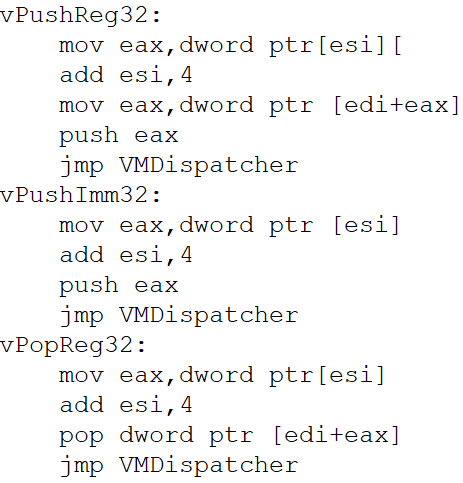
\includegraphics[height=7cm]{fuzhu.png}
	\bicaption{辅助Handler执行核心代码}{The helper Handler executes the core code}
	\label{fuzhu}
\end{figure}

\subsubsection{普通Handler}

\label{normalhandler}
在图\ref{fuzhu}的基础上,可以实现普通指令Handler,其实现代码如图\ref{normal}所示。

\begin{figure}[htbp]
	\centering
	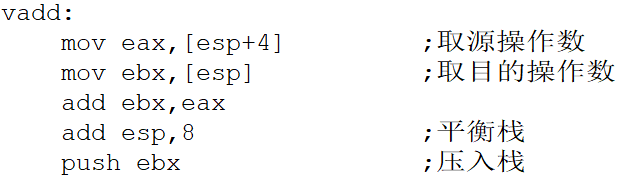
\includegraphics[height=2.5cm]{normal.png}
	\bicaption{普通Handler执行核心代码}{The normal Handler executes core code}
	\label{normal}
\end{figure}


将一个普通的汇编指令分为两个部分进行,指令的实现由普通Handler处理,目的操作数和源操作数都交由栈Handler处理。这样可以用更少的模拟Handler实现真正的汇编指令。

举一个例子便于理解。例如,sub指令的形式通常有“sub reg,imm”,“sub reg,reg”,“sub mem,reg”等,这里采用现将两个操作数使用栈Handler处理,将两个操作数存放在栈中,然后再调用“vsub Handler”,在这时两个操作数已经以立即数的形式在栈中,则“vsub Handler”可以直接默认栈顶就存放着它需要处理的数据,接着可以直接对栈顶这两个立即数进行减操作。
%vsubHandler的汇编代码如下。

%图

%再给出两个转换过程的伪代码,如下

%sub命令转化

%图1 图2 
%p744

%

\subsection{多样化Hanlder实现}

本课题的核心保护模块则是使用了多样化Handler模块,所谓多样化,就是将同一个Handler功能的模块采用多种设计方案,比如转移指令、算术指令、CALL指令等,由于汇编语言的特性,往往相同的功能可以采用多用方式实现,一旦相同功能采用不同汇编代码实现,逆向攻击者在分析虚拟机时会得到不同的Handler结果,并且每次分析的结果可能都不一样,使得逆向攻击者不能获得正确的Handler,也就无法掌握由汇编代码到字节码的翻译过程,通过这种方式,可以有效加大逆向攻击者的逆向分析难度。

\subsubsection{转移指令多样化}

转移指令一共包括四种指令,分别是无条件转移、条件转移、CALL和RETN。

由于无条件转移在汇编语句中就是JMP指令,而JMP指令的核心实现就是改变寄存器EIP的值无条件跳转指令JMP的Handler比较简单,如图\ref{jmpzhiling}所示。

\begin{figure}[htbp]
	\centering
	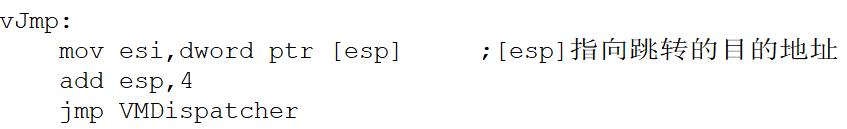
\includegraphics[width=13cm]{jmpzhiling.png}
	\bicaption{jmp的Handler实现代码}{The Handler implementation code for JMP}
	\label{jmpzhiling}
\end{figure}


JMP指令的功能太过单一,多样化的实现意义不大,所以本节将会介绍条件转移的多样化方法。X86的条件转移指令和条件传输指令是可以通过某种方式对应起来的,其比较如表\ref{jmp}所示。

\begin{table}[htbp]
	\bicaption{条件转移指令和条件传输指令}{Conditional transfer instruction and conditional transfer instruction}
	\begin{tabular}{c|c}
		
		\hline
		条件转移指令 & 条件传输指令 \\ \hline
		jne    & cmovne \\ \hline
		ja     & cmova  \\ \hline
		jb     & comvae \\ \hline
		jbe    & comvbe \\ \hline
		je     & comve  \\ \hline
		jg     & comvg  \\ \hline
	\end{tabular}
	\centering

	\label{jmp}
\end{table}
所有条件跳转指令都有对应的条件传输指令,图\ref{jne}是通过设计之后,条件跳转指令和条件传输指令的实现方法。

\begin{figure}[htbp]
	\centering
	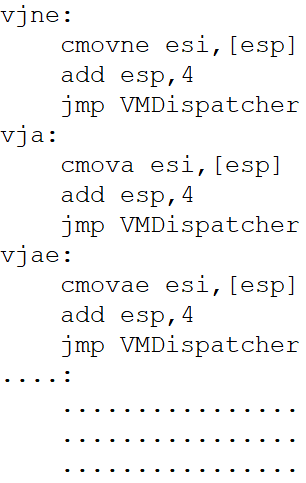
\includegraphics[width=5cm]{jne.png}
	\bicaption{条件跳转指令的另一种实现}{Another implementation of conditional jump instruction}
	\label{jne}
\end{figure}


这里再提出一种方式实现转移指令多样化,可以使用X86平台下的标志寄存器和无条件转移指令实现另一种跳转命令模拟跳转,原理是条件转移命令本身就是判断标志寄存器中的值实现跳转的,而存在其他指令可以直接读取标志寄存器的值,直接判断标志寄存器中的值,加上无条件跳转JMP的配合,就可以实现条件跳转。

%这里以JAE指令为例,代码如下。

%图746

%下图是伪代码的调用。

%vPush jmpto add adfa 
%d
%sdf
%adfa
%sdf

%上述过程为,首先读取标志位,根据取得的值(CF位)和1做and运算。使用CMOVE指令判断ZF标志位是否为0,如果为0就改变ESI的值。JAE指令只判断CF位。

%再举一个JBE指令的例子,Handler的汇编代码如下。

%图

%通过JAE指令和JBE指令的举例,实现了同一个Handler指令的多种实现方式,其他条件跳转指令转化原理基本一致,这里不再举例。

\subsubsection{算术指令多样化}


在X86指令体系中存在一些不同指令可以用同一种指令去实现的情况,它们的目的都是将esi指令加一,但是却是inc指令和add指令的不同实现方式,示例代码图\ref{add}所示。


\begin{figure}[htbp]
	\centering
	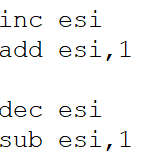
\includegraphics[width=2.3cm]{add.png}
	\bicaption{add指令和sub指令的另一种形式}{Another form of the Add and SUB directives}
	\label{add}
\end{figure}


X86体系中存在很多这种指令,实现原理于图\ref{add}类似,在Handler多样化实现时都可以利用这种机制,实现汇编到字节码翻译过程中的Hanlder指令多样化。

具体操作方式则是如\ref{normalhandler}节所述,将操作指令、目的操作数、源操作数分别使用不同的Handler实现。


\subsubsection{CALL指令多样化}

CALL指令虽然作为跳转指令的一种,但在功能实现方面与JMP衍生出来的指令大不相同,CALL指令通常是调用一个函数,虚拟机中的代码运行通常在一个栈中进行,但是CALL指令由于是进到另外一个函数中执行,所以会需要把控制权交给真实的CPU,举例代码如图\ref{call1}所示。

\begin{figure}[htbp]
	\centering
	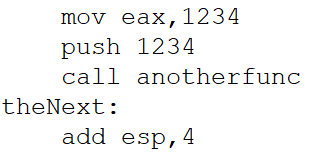
\includegraphics[width=5cm]{call.png}
	\bicaption{call指令示例汇编代码}{Call instruction sample assembly code}
	\label{call1}
\end{figure}

除第三条指令外,其他指令都是在一个栈层次上进行,不需要更换栈,但是第三条指令“CALL anotherfunc”是对其他函数的调用,它的栈帧会改变,所以必须将控制权交给其他代码。

汇编语言中,CALL指令先把当前执行指令的下一条指令压入栈中,然后再跳转到目标函数的首地址处,代码如图\ref{a}所示,将控制权交给其他代码之后必须再跳回虚拟机中,所以使用代码如图\ref{b}所示,这是返回虚拟的一段代码,NextCode代表THEnext之后代码的字节码。只需要将thenext的地址修改为nextVM的地址,便可以再次模拟一个CALL指令,vcall指令的伪代码如图\ref{c}所示。


\begin{figure}[htbp]
	\centering
	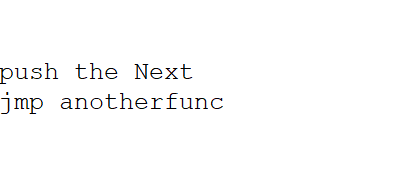
\includegraphics[width=6cm]{a.png}
	\bicaption{目标函数的首地址}{The starting address of the target function}
	\label{a}
\end{figure}

\begin{figure}[htbp]
	\centering
	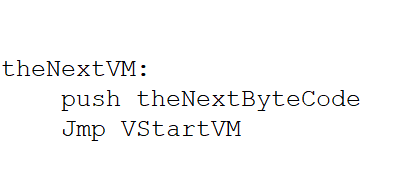
\includegraphics[width=6cm]{b.png}
	\bicaption{跳回虚拟机代码}{Jump back to the virtual machine code}
	\label{b}
\end{figure}

\begin{figure}[htbp]
	\centering
	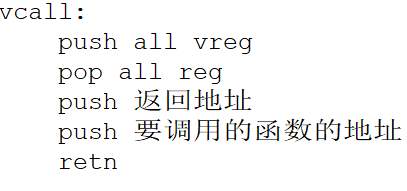
\includegraphics[width=6cm]{c.png}
	\bicaption{vcall指令的伪代码}{The pseudocode for the VCall directive}
	\label{c}
\end{figure}



\section{本章小结}
本章采用虚拟机保护的方法对Windows下可执行文件进行了保护,并提出一种多样化Handler设计思路,实现了该方法,对转移指令、算术指令、CALL指令进行了多样化设计,由于X86架构和汇编语言的特性,指令本身的实现不是唯一的,将Handler分为辅助Handler和普通Handler,以低耦合的特点设计了汇编语言和字节码之间的转换协议,本章的试验将会在后文进行详细描述。
\chapter{静态分析混淆技术研究与实现}
%第四章内容
逆向攻击者在分析软件时通常会通过动态分析工具如OllyDbg、WinDbg、SoftICE等工具和静态分析工具如IDA工具来分析软件,动态分析工具是在运行是分析可执行程序,可以观察到程序执行时的寄存器、堆栈、内存空间等的所有数据。静态分析工具则是直接反汇编源码,它的优点是对代码阅读者提供更多的信息,高级功能的静态分析工具比如IDA甚至可以直接由汇编代码得到与源码类似的C语言代码,函数的所有跳转都给出详细信息。

本节将针对静态分析工具对软件进行反调试保护,提出一种建立索引进行函数间基本块交换的混淆算法,最后根据提出的算法实现了一个PE文件保护器。
\section{常用的反调试技术}
\label{cha2:sec:techarch}

常见的反调试技术有使用花指令、文件完整性检验、代码与数据结合、调试器检测等。

逆向工程是研究程序以获得有关其工作方式和使用的算法的封闭信息的过程,尽管软件逆向可用于合法的研究目的,尤其是恶意软件分析或未记录的系统研究,但通常认为是黑客将其用于非法活动,调试与反调试一直都是软件保护者和软件破解者之间的相互博弈,虽然理论上不存在不能被逆向分析破解的程序,但是软件保护者们依然采用各种各样的方式来实现对软件的保护,逆向工程的工作中也没有最优解。本课题也只是在加大破解难度的原则上对软件进行保护,并加入自己的加密算法,最终加大破解难度或者引导破解者到错误的方向。本节将简述常见的的基本保护措施,并会加以改进。

常见的分析软件的方法有:一、使用数据包嗅探器进行数据交换分析,以分析通过网络交换的数据。二、软件二进制代码反汇编以汇编语言形式列出其代码。三、反编译二进制或字节代码,以高级编程语言重新创建源代码。本课题考虑了流行的反破解和反逆向工程保护技术,即Windows中的反调试方法。我们一开始就应该提到,不可能完全保护软件免受逆向工程。各种反逆向工程技术的主要目标只是使过程尽可能复杂。

\subsection{花指令}

花指令是一种隐藏不需要进行反向工程的代码块或其他功能的方法。在实际代码中插入一些垃圾代码还可以确保原始程序的正确执行,并且程序无法很好地进行反编译,难以理解程序的内容并难以达到使代码混乱的效果,使用某种方式排布数据和代码,在汇编代码中插入一些“数据垃圾”,对反汇编软件进行干扰。

第一种花指令利用了汇编指令的长度。不同的体系结构的机器指令长度并不相同,有多操作码指令和单操作码指令的区分,多操作码指令需要确定这条指令第一个字节的起始位置,由于长度固定,所以指令的结尾也是固定的,否则可能会被反编译器翻译为其他的或者错误的指令。图\ref{huazhilinga}是一段汇编代码。

\begin{figure}[htbp]
	\centering
	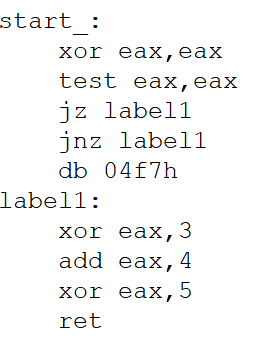
\includegraphics[width=4cm]{huazhiling.png}
	\bicaption{花指令汇编源码}{Flower instruction assembly source code}
	\label{huazhilinga}
\end{figure}


对源程序使用nasm编译,使用W32Dasm反汇编,结果图\ref{huazhliingb}。

\begin{figure}[htbp]
	\centering
	\centering
	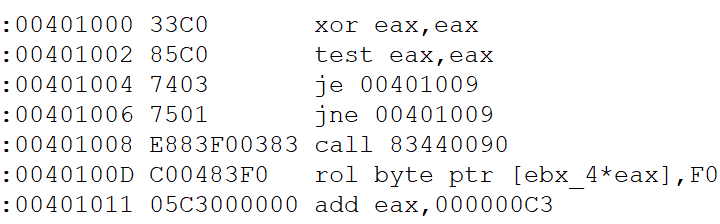
\includegraphics[width=10cm]{huazhilingb.png}
	\bicaption{反汇编硬编码代码}{Disassemble hardcoded code}
	\label{huazhliingb}
\end{figure}

W32Dasm使用的反汇编器是逐行反汇编的,代码中的04F7h不是任何汇编指令,干扰了W32Dasm使用的Linear Sweep反汇编引擎,对指令的起始位置做出了错误的判断,使反汇编的跳转指令的跳转位置无效。比如00401009h这个位置属于指令的内部,不具有反花指令引擎的反汇编器很容易给调试者带来无效的分析信息。

反汇编引擎最关键的问题之一是代码与数据的区分,由于汇编代码的指令长度是不同的,并且代码之间存在绝对地址和相对地址,跳转命令可能使用这些地址来直接跳转或间接跳转,所有反汇编引擎要对所有指令的长度和功能有确切的认知,从而保证反汇编结果正确性。

第二种花指令是利用了将JMP指令修改为JE+JNE(JX+JNX或者JZ+JNZ等)实现的。

在汇编语言中存在着大量的条件跳转,比如JNE是比较两个操作数,如果不相同,则跳转,如果不同,则不跳转,JE与上述指令功能相反。条件跳转都是成对出现的,比如JZ/JNZ、JX/JNX等。而JMP指令则是无条件跳转,使用方法为JMP XXXX,指令运行时永远会跳转到XXXX处,JMP这条指令的地址和XXXX代表的地址中间的代码可能永远不会被执行,这部分代码叫做DEAD CODE。JE+JNE型代码与JMP代码同理,如果将JE和JNE代码同时使用,将会实现无条件跳转。

\begin{figure}[htbp]
	\centering
	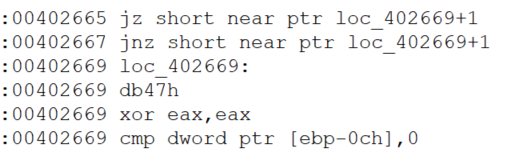
\includegraphics[width=9cm]{jnz.png}
	\bicaption{跳转花指令}{Jump flower instruction}
	\label{jnz}
\end{figure}


如图\ref{jnz}所示,无论标志位是否为1,代码都会跳转到00402669处执行,代码都会跳转到00402669处执行 47h指令,也就是无用代码。db 47h指令则会给反编译器带来困扰,因为这行代码是在代码区域,但是不能被识别为指令。

第三种花指令的抗逆向效果较低,但是这部分指令不会影响其他部分有用程序,对程序的影响较小,植入的成本更低,程序不容易出现错误。这种花指令通常构造一部分没有意义的算术运算。

%第一行和第二行都是EBX加2,第五行EBX加上1,第七行EBX减1,所以EBX的值并没有发生变化;第三行的NOP,无意义代码;第四行EAX加28,第六行EAX加上负28,所以EAX的值也没有被改变。这种垃圾指令是最常见的花指令,通常可以使用脚本自动去除这种花指令,干扰的效果较低,但是如果添加大量的这种指令仍然可以给逆向分析者带来麻烦。

\subsection{文件完整性检验}

在抗逆向方案中,文件完整性检验是最基础的方案,通常也被最先考虑并采用。文件完整性检验就是在软件运行过程中,对本文件进行自身完整性的检查,抵御逆向分析者对文件进行修改,可以达到一定的抗分析目的。

文件完整性检验原理就是在发布时预先计算文件的哈希值,存放在程序的启动代码中,在文件每次运行时,首先对当前文件的某个模块或者全部模块进行哈希运算得出哈希值,与预先计算好的哈希值对比,如果相同则成功执行,如果不同则直接终止程序。

文件完整性检验通常使用三种方式,分别是:磁盘文件校验的实现、内存映像校验和校验和。

其中的校验和方式安全性能较差,在PE文件的IMAGE\_OPTIONAL\_HEADER中有一个校验和(Checksum)字段,这个数据结构中已经存放着整个文件的校验和,相当于PE文件对自身的一种保护,但由于这种保护广为人知,现在几乎已经失去它的作用,只要逆向分析者发现有校验和的检查,自己手动修复校验和或者使用工具修复都可以成功绕开这个限制。
%Windows提供了一个API函数来检测校验和,其原型如下图

%图657

%\subsection{常量分解}

%常量分解就是对一些寄存器中存储的常数值进行展开,对常数进行分解,可以使程序的运行更加复杂,在下图 中 两条指令分别是将3赋值给EBX和将4096赋值给EDX。4096字节为4K,大小为一个页。如图a中4096可以得出这段代码很可能是4K大小的一个数组。图b为图a的展开后的结果,第一行指令将1000赋值给EBX,第二行加16后EBX等于1016,第三行将EBX逻辑右移9位,1016向逻辑右移动9位后刚好位1;第四行将1赋值给EDX,然后将第五行将EDX逻辑左移12位,正好是4096大小。

%图

%常量展开就是将常量以一种复杂的方式再计算一遍,最后的结果相同,虽然这样会加大程序的运行时间,并且实现的复杂度比较高,不利于代码的优化,但也一定程度上影响逆向分析者的工作量。


\subsection{调试器检测}

\subsubsection{使用IsDebuggerPresent}

提出的反调试方法是基于IsDebuggerPresent函数。此函数检测调用模式是否正在由用户模式调试器调试。图\ref{isdebug}的代码显示了基本保护的示例:

\begin{figure}[htbp]
	\centering
	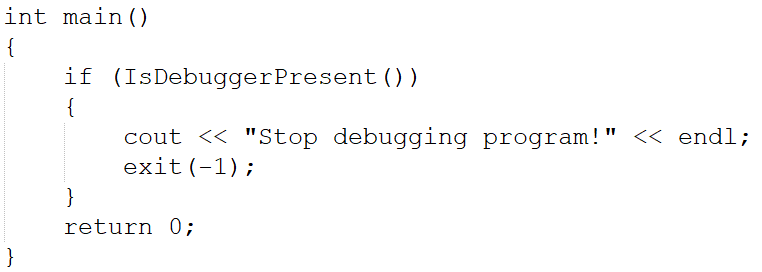
\includegraphics[width=10cm]{isdebug.png}
	\bicaption{IsDebuggerPresent函数}{IsDebuggerPresent function}
	\label{isdebug}
\end{figure}

%如果看一下IsDebuggerPresent函数内部,将会发现一下代码:

%\begin{lstlisting}
	
%	0:000< u kernelbase!IsDebuggerPresent L3
%	KERNELBASE!IsDebuggerPresent:
%	751ca8d0 64a130000000    mov     eax,dword ptr fs:[00000030h]
%	751ca8d6 0fb64002        movzx   eax,byte ptr [eax+2]
%	751ca8da c3              ret
%\end{lstlisting}

%对于X64进程

%\begin{lstlisting}
%	0:000< u kernelbase!IsDebuggerPresent L3
%	KERNELBASE!IsDebuggerPresent:
%	00007ffc`ab6c1aa0 65488b042560000000 mov   rax,qword ptr gs:[60h]
%	00007ffc`ab6c1aa9 0fb64002           movzx eax,byte ptr [rax+2]
%	00007ffc`ab6c1aad c3                 ret
%\end{lstlisting}

%PEB(过程环境块)结构相对于fs段偏移了30h(对于x64系统,相对于gs段偏移了60h)。如果我们查看PEB中的2偏移量,则会发现该BeingDebugged字段:

%\begin{lstlisting}
	
%	0:000< dt _PEB
%	ntdll!_PEB
%	+0x000 InheritedAddressSpace : UChar
%	+0x001 ReadImageFileExecOptions : UChar
%	+0x002 BeingDebugged    : UChar 
%\end{lstlisting}

\section{建立索引进行函数间基本块交换的混淆算法}

本节将会提出一种对混淆算法,此算法对二进制函数分块,进行交换,并建立函数块之间交换记录的索引。目前市面上大部分混淆算法都是对一个函数的二进制进行加密处理,比如对函数内部的汇编代码进行花指令处理或进行分块然后进行交换。由于函数内部的二进制代码可能极其复杂,函数之间进行块交换的主要困难在这几个方面:一、编程难度大,由于只能看到函数的二进制代码;二、虽然通过反汇编处理后可以看到汇编代码,但是在编程时需要分析各条指令的长度、函数执行时的栈帧结构的保护、执行时内存堆空间的变化情况。

本节将会提出相对简单的二进制混淆方式,只考虑移动函数内部二进制命令中较易处理的汇编命令,比如MOV、SUB、ADD等不影响栈和堆的汇编指令,且这些指令的长度大部分是固定的,后文将会实现这种算法,并进行分析。

\subsection{基本思想} 

一个可执行程序中包含多个函数,函数之间可能进行相互调用,首先要对函数进行分块处理,把每个函数切分为可交换块和不可交换块,可交换块数量大于等于一,在移动时只会移动可交换块,故不考虑不可交换块块数。通常,函数的指令都是连续的,函数的调用流程反映了程序的执行时的运行结构。

在记录交换索引的基础上,对函数之间的可交换块进行了的交换,在可执行文件的尾部建立一个新节来存储索引信息。

\begin{figure}[htbp]
	\centering
	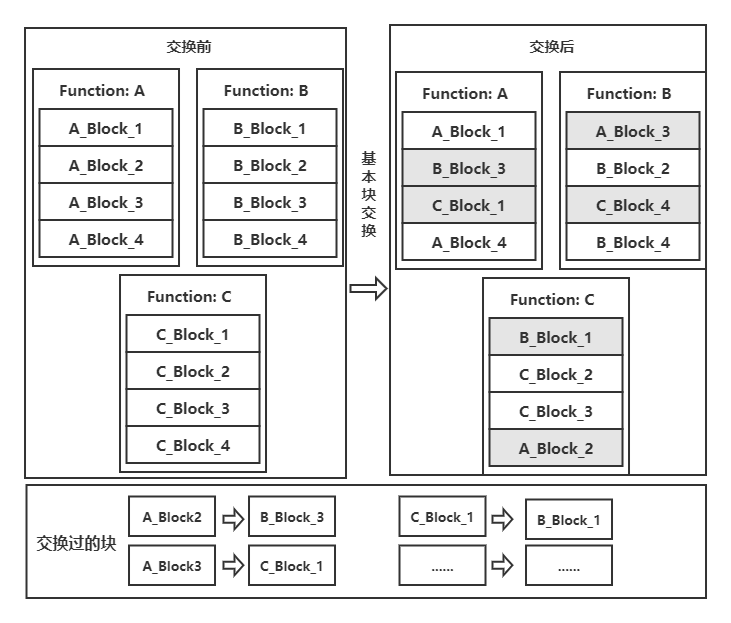
\includegraphics[width=13cm]{switch.png}
	\bicaption{建立索引进行函数间基本块交换过程}{Establish an index for the basic block exchange process between functions}
	\label{switch}
\end{figure}

如图\ref{switch}所示,图中展示了三个函数块的交换过程,并在左侧建立索引,在恢复时程序会根据此索引进行函数执行流程恢复。函数X、Y、Z分别包含了4个基本块,函数X的基本块X\_Block\_2、X\_Block\_3、函数Y的基本块Y\_Block\_1、Y\_Block\_3、函数Z的基本块Z\_Block\_1和Z\_Block\_4参与了交换,基本块Y\_Block\_3和C\_Block\_1被交换到了函数X中、基本块X\_Block\_3和Z\_Block\_4被交换到了函数Y中、基本块B\_Block\_2和A\_Block\_2被交换到了函数Z中。根据图\ref{switch}右半部分所示,在程序执行时,解释器需要根据索引情况确定被交换过的块。

建立索引进行函数间基本块交换的混淆算法的基本思想是将某个函数的可交换块,通常是MOV、ADD、SUB等不影响堆栈和内存的指令块和其他函数的可交换块进行交换,并使用索引记录的方式记录交换情况,在索引方面,也要使用相关的指令使程序在正常运行时保证在正常运行时可以正常还原。在索引的位置也要进行相关的操作,索引的开头位置使用PUSHAD指令进行寄存器的保护,在索引的结束位置使用POPAD进行寄存器的恢复操作。PUSHAD指令的功能是将目前所有的寄存器指令压入栈中,POPAD指令则是PUSHAD指令的逆操作。混淆后的函数控制信息被隐藏到了索引中,所以每一条索引都包含了两个函数的交换块信息。

静态分析工具都是以函数为基本单位进行二进制分析,当使用静态分析工具分析经过此种方式加密的程序时,会产生分析函数失败的各种不可预料的错误,大大的加大了静态分析难度,增加了逆向分析者的分析时间和代价。

\subsection{算法描述}

假设加密程序P由多个函数F1、F2...Fn组成,对程序P进行反汇编处理,得到程序P中的一系列函数信息。在这些函数中选取部分函数,并将函数进行基本块分割,将函数分为A、B、C、D、...,根据每个组内的函数数量,将随机选择函数放入多个小组中。A0中包含m个函数$f_{0} $、$ f_{1} $、…、 $ f_{i} $、…、$ f_{m-1} $ ,从函数$ f_{i} $(i$\in$[0,m-1])中选取n个基本块,然后将参与混淆的基本块进行随机交换。

基本块交换的形式化定义:参与的函数为$ f_{i} $(i$\in$[0,m-1]),每个函数内参与的基本块为$ B_{ij} $(i$\in$[0,m-1],j$\in$[0,n-1]),然后对这些基本块进行随机处理,最初基本块$ B_{ij} $(i$\in$[0,m-1],j$\in$[0,n-1]),随机处理改为$ B_{k,l} $(k
$\in$[0,m-1],l$\in$[0,n-1])。

根据上述形式化描述可知,基本块的交换相当于对二维数组的随机打乱处理。假设参与的函数有四个,所有函数参数的函数数量也为四个,那么交换之前基本块的位置如表\ref{qian}所示。

\begin{table}[htbp]
	\centering
	\begin{tabular}{ccccc}
		\hline
		交换前位置 & 0    & 1    & 2    & 3    \\ \hline
		f0    & B0   & B0,1 & B0,2 & B0,3 \\
		f1    & B1,0 & B1,1 & B1,2 & B1,3 \\
		f2    & B2,0 & B2,1 & B2,2 & B2,3 \\
		f3    & B3,0 & B3,1 & B2,3 & B3,3 \\ \hline
	\end{tabular}
	\bicaption{基本块交换前位置}{Position before basic block exchange}
	\label{qian}
\end{table}

其中基本块的序号表示此基本块的函数在所处函数参与交换的基本块的索引位置,设定0为基本块的起始位置。混淆算法的目的是将上表中$B_{i,j}$(i$\in$[0,3],j$\in$[0,3])进行随机打乱,得到一个新的二维数组,可以假设打乱后的结果如表\ref{hou}所示。

\begin{table}[htbp]
	\centering
	\bicaption{基本块交换后位置}{Position after basic block exchange}
	\begin{tabular}{ccccc}
		\hline
		交换前位置 & 0    & 1    & 2    & 3    \\ \hline
		f0    & B2,1 & B2,1 & B1,3 & B1,1 \\
		f1    & B3,0 & B0,2 & B1,0 & B3,2 \\
		f2    & B1,2 & B0,3 & B0,0 & B3,1 \\
		f3    & B0,1 & B3,3 & B2,3 & B2,2 \\ \hline
	\end{tabular}

	\label{hou}
\end{table}

这里使用Knuth-DurstenfeldShuffle一维数据随机化算法,这里首先将二维数组一维化,将数组a[m][n]转化为a[m*n],通过上述的方式,将二维数组内的数据转化为一维数组内的随机数据。在最后,再进行一维数组二维化,也就是上述操作的逆操作。


\section{二进制混淆器设计与实现}

根据上一节提出的二进制混淆算法,本节设计并实现二进制混淆器。

\subsection{总体设计}

改加壳机制总体架构如图\ref{hunxiaoqi}所示。加壳器主要由四个模块构成,分别为反汇编引擎、控制流程、索引建立和加密混淆引擎、文件重建。

\begin{figure}[htbp]
	\centering
	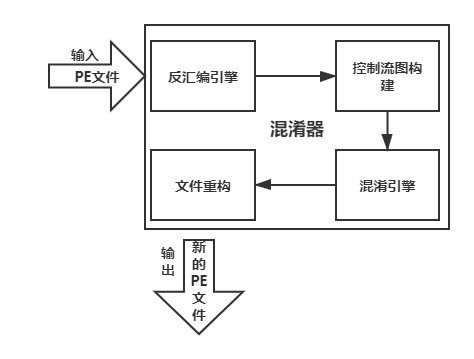
\includegraphics[width=8cm]{hunxiaoqi.png}
	\bicaption{混淆器总体结构}{The overall structure of the obfuscator}
	\label{hunxiaoqi}
\end{figure}

加壳器的输入为PE文件,输出为加壳后的PE文件。反汇编引擎模块对输入的PE文件进行反汇编,得到汇编代码;索引和控制流程把通过反汇编引擎得到的数据进行分析,处理程序的可交换函数、函数之间的调用情况、基本块的数量等信息;加密混淆引擎是整个处理流程的核心,根据索引和控制流程的信息,对程序进行函数混淆加密;文件重建是对混淆后的数据进行重构输出新的PE文件。

\subsection{二进制分析器设计与实现}
\label{san}

本节主要的内容是使用反汇编引擎对PE文件进行静态分析,为下节混淆器进行加密做准备。反汇编引擎使用OllyDbg的反汇编引擎,这个反汇编器是开源的,速度快,易于使用且稳定。由于本文提出的二进制混淆算法只处理MOV、SUB、ADD等不涉及堆栈和内存的混淆,属于非常基本混淆机制,没有复杂的内存处理,所有使用本反汇编引擎是最好的选择。

控制流程最主要的任务是建立基本块,如图\ref{jibenkuai}所示。

\begin{figure}[htbp]
	\centering
	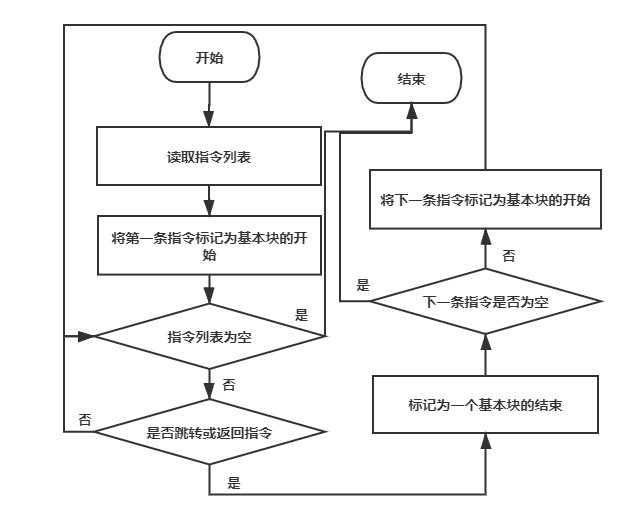
\includegraphics[width=11cm]{jibenkuai.png}
	\bicaption{基本块的识别过程}{Basic block recognition process}
	\label{jibenkuai}
\end{figure}

基本块的识别流程为:1.读取所有指令,标记起始指令;2.遍历指令列表,判断当前指令是否为返回指令或者跳转指令;3.如果不是跳转或返回指令则执行步骤2,进行下一条指令的遍历,否则将标记为基本块的结束;4.将下一条指令标记为另一个基本块的开始,跳转到2继续遍历其他所有指令。


\subsection{混淆器的设计与实现}


混淆器的编程实现难度偏高,故本文的实现中所参与交换的函数,不涉及处理内存、堆和栈中的数据,只处理交换函数之间的MOV、SUB、ADD等寄存器变换的指令。本文为了方便实现,将算法的某些细节进行简化,算法将不对函数进行详细分组,直接使用随机算法进行满足要求的函数,其中可能包含大量的MOV、SUB、ADD等基础指令并进行混淆。

\begin{figure}[htbp]
	\centering
	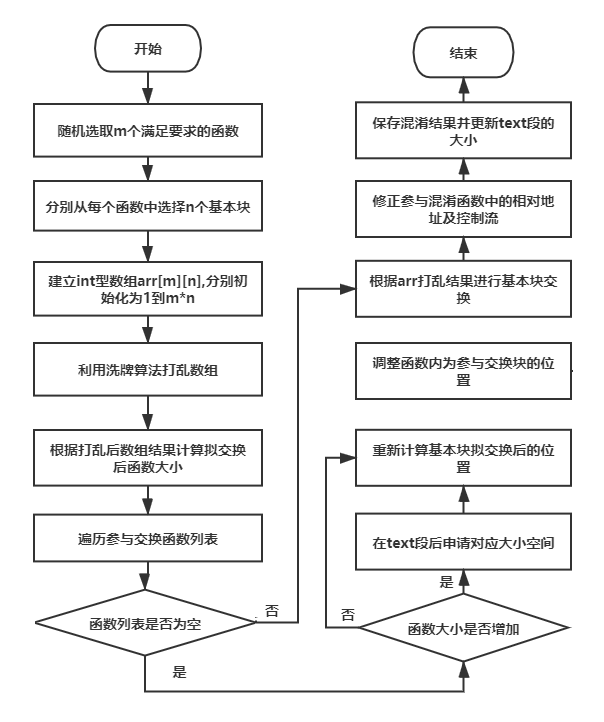
\includegraphics[width=13cm]{hunxiaoyinqing.png}
	\bicaption{混淆引擎工作原理}{How the obfuscation engine works}
	\label{hunxiaoyinqing}
\end{figure}

混淆器的工作流程如图\ref{hunxiaoyinqing},具体流程为:1.加密引擎首先根据二进制分析器提供的构建信息,从满足要求的函数中随机选取m个函数;2.将m个中选出的函数进行n个基本块之间的交换;3.建立一个long型数组arr[m*n],并进行1-m*n的初始化。4.使用Knuth\_Durstenfeld Shuffle算法对数组arr随机化;5.将函数产生的随机化数据进行如实交换;6.遍历参与混淆函数列表,如果为空,转到步骤11;7.判断函数的占用空间变化情况,如果没有变大,跳转到步骤9,否则在PE文件的最后加一个add节,并申请所需空间;9.计算出各个基本块交换后的新的位置,同时将交换索引放到PE文件中的add节中;10.保存处理过的指令,这里只处理了MOV指令;11.将arr数组的结果放到新的位置;12.修正函数的相对地址;13.保存混淆结果更新PE文件头,计算新添加节表的大小,并添加新add节表。

\subsection{二进制文件重建}

PE文件的重建工作是设计加壳器的重要一环,也是编程的瓶颈所在,PE文件重建,是根据加密结构重新建立一个PE文件,需要用到第二章提到过的大量内容。首先,肯定不能将混淆之后的汇编代码直接放到PE文件的各个段中,因为PE文件的各个段在经过加密之后占用空间大小会有所增加,PE文件头部的各个段大小需要修改。另外,各个段起始位置也都需要修改,否则可能会出现两个段重合。段中的跳转地址也需要相应的修复操作。将以上的信息进行修正之后,才能将修改后的汇编代码翻译成机器码写入到text段中重新生成一个PE文件。

%PE文件的重建模块流程如下图

%图
%所示。

PE文件重建步骤为:1.将混淆后的结果翻译成机器码,计算混合后的各个段的占用空间;2.更新PE文件头PE可选头表;3.检查混淆后代码段是否产生重叠,如果不重叠跳转到步骤5;4.将重叠的段向后移动;5.按照PE文件的布局依次将混淆后的结果依次写入到新的PE文件中,保存文件并退出。


%在面对软件保护技术的过程中由于许多软件开发人员仅专注于软件系统功能的实现,因此他们忽略了软件加密保护和反向破解。因此,在研究软件保护的初期,研究人员开发了一些相对有用的专业软件加密保护程序(简称Shell)。但是,随着破解技术的发展,甚至可以使用免费的OllyDbg删除使用强大的加密算法(例如Twofish,TEA,Blowfish以及CRC(循环冗余校验)和反调试技术的组合)的坚固外壳ASProtect。动态跟踪外壳后的反汇编代码。使用堆栈平衡原理在程序执行入口之前找到外壳,然后结合LoadPE工具的强大功能来导入表,导入地址表和重定位表。市面上大部分对软件的保护都基于上述的几种方式,本文将会在已有反调试基础上对已有算法进行优化改进。

%本课题实现的目标是对软件进行保护,防止未授权用户的非法注册,将分为两个大的设计模块,一方面对软件加入反跟踪调试技术,并对在目前流行的反跟踪调试基础上加入新的算法,以实现对非法用户的反编译混淆,另一方面对软件整体进行虚拟机加壳的方式进行保护,并在已有虚拟机Hanlder加密基础上进行动态加密解密,虚拟机加壳的方式是目前安全性能最高的方式,但是由于虚拟机保护方式需要在受保护的程序中加入虚拟机中字节码的解释器,因此在运行过程中会消耗大量的CPU时间,本文也会对加密后的程序的运行时间进行优化处理,尽可能提高程序的运行速度,并对已有虚拟机加壳进行对比。


%在试验阶段,将会使用不同的反编译器ODDBG、IDA、WinDbg)对加壳后的程序进行反汇编,对反调试性能和程序运行速度与市面流行保护引擎进行对比。由于Linux和Windows操作系统的PE(Portable Executable)文件结构完全不同,本课题的所有实验环境仅限于Windows操作系统下的PE文件,对Linux下的ELF文件并不能进行加壳保护。

%本文的主题是围绕反调试技术和虚拟机加壳技术,从用户角度和破解者角度分别给出不同情况的分析方案,并基于此建立了一个软件保护框架,为反调试技术提供良好的试验环境。整体的框架结构参考图~\ref{cha2:fig:framework}。其中自下而上,按照颜色划分,黄色:操作系统内核层,黄色:操作系统PE文件装载器,蓝色下层:逆向技术(动态分析、静态分析)和PE文件结构,蓝色上层:反跟踪技术和软件加壳(加密壳、虚拟机壳),绿色:用户接口API。除了操作系统层之外,每部分都将在后文依次介绍。


\label{cha2:sec:arch}

%软件工程中软件架构是整个系统的草图,在本节中,基于上面图~\ref{cha2:fig:framework}中所给出的结构中的操作系统PE文件装载器和Windows kernel层加以分析,并根据逆向分析技术和PE文件结构这两个层面分别阐述我们要实现的反调试算法架构设计。反调试是在应用程序代码内使用的一组技术,用于检测和阻止调试行为。这阻止了攻击者动态运行应用程序,试图了解它们的工作方式并更改应用程序内某些功能或检查的行为。反调试技术包括观察和检测内存,操作系统,进程信息以及将调试器连接到应用程序后与没有调试器时相比出现的延迟之间的细微差异。尽管有几种不同的反调试方法,但是使用的主要方法之一就是修改后的代码反调试。该技术将代码插入应用程序的多个位置,以主动搜索断点,调试器或调试技术。这些断点的检测可以通过分析整个应用程序操作过程中的代码修改,同时将其与预期值或规范进行比较来获得。检测到的差异会引发警报,从而可能导致更深入的调查。


\section{本章小结}

本章对常见的静态分析混淆技术进行了研究,对抗逆向中容易出现的问题进行了总结,分析了已有方法的优缺点,并提出一种建立函数索引进行函数间基本块交换的一种混淆方式,基于随机算法的二进制代码混淆算法,对算法的细节进行了详细的描述。最后根据提出的算法设计并实现了一个PE文件加壳器,本文实现了MOV、SUB、ADD等指令的交换方式在处理内存和堆栈区域上,在进行混淆之后,合理地还原程序的运行环境,就可以实现其他指令转化方法。










\chapter{系统实现与测试}

本章将实现的PE文件虚拟机加壳和PE文件二进制混淆器组装成一个PE文件保护系统,并分别对本系统的保护壳和加密壳进行了功能验证、加密性能评估。其中本系统虚拟机壳的多样化Handler是在已有的虚拟机壳进行修改,并进行了Handler多样化的改进,增加了加壳后文件二进制编码的多样性,对逆向攻击者进行了有效的误导,二进制混淆器针对静态调试器进行防御,提出一种对函数间基本块交换的混淆算法,并记录交换块的索引放到文件的最后节表中,但由于交换函数间指令后修复程序的运行环境如内存、堆、栈、寄存器等难度太高,本文将针对MOV、SUB、ADD等不影响堆栈的指令进行交换,其余指令在保证能够恢复运行时的环境也可以实现,本章将会对以上的动态和静态保护措施进行实现和测试。


\section{总体设计方案}

\subsection{编程语言的选择}

通常情况下PE文件二进制保护软件使用C语言或者汇编来编写,市面流行的加密壳的外壳部分通常使用汇编代码,使用汇编语言编写,可以实现更加复杂的算法并且对PE文件的二进制混淆算法更容易实现,但是汇编语言难以掌握,并且通常情况下不具有可移植性,所以本保护系统将会使用C++和汇编语言编译器为X86nasm混合编程的方式,在需要对PE文件加壳的复杂位置使用汇编语言,程序的整体架构采用C++,这极大地提高了开发效率和降低了开发难度。

\subsection{软件的系统构架}

本系统采用模块化设计有利于系统的开发和维护,采用模块化结构有利于对软件功能进行细分,模块出现问题更利于修改。本系统有以下几个模块构成:外壳添加模块、反调试模块、特殊数据处理模块、区块压缩模块、输入表构建模块、反静态分析模块、虚拟机模块、PE文件读取模块组成。其中反调试模块、区块压缩模块、虚拟机模块采用汇编语言编写,采用X86nasm编译器。

\section{功能验证}

功能测试部分将对系统中的虚拟机加密和二进制混淆器的功能分别进行测试。在32位Windows 10系统下磁盘空间为120G、内存为2G的环境下进行功能测试,选择32位PE文件notepad.exe作为测试文件。在未进行虚拟机加密或未经二进制混淆之前,程序Aseprite.exe的运行情况如图\ref{aseprite}所示。

\begin{figure}[htbp]
	\centering
	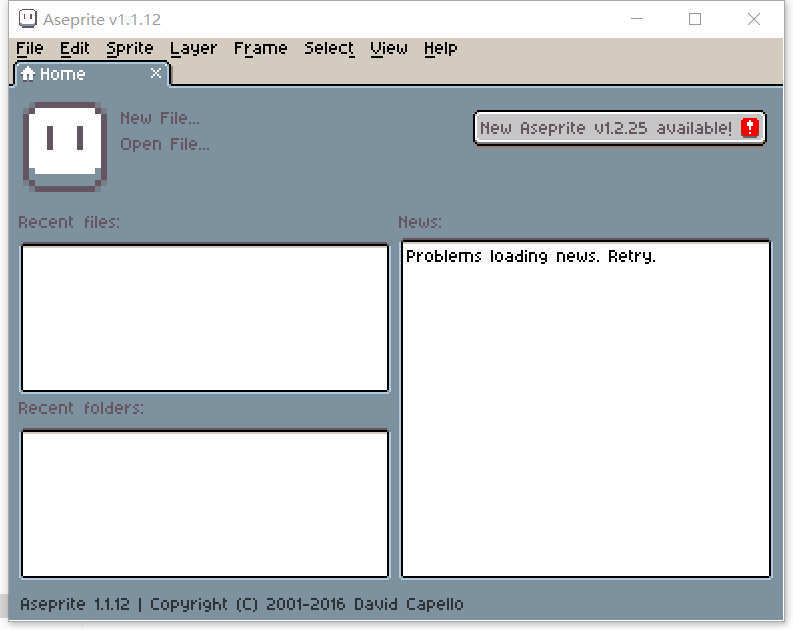
\includegraphics[width=10cm]{aseprite.png}
	\bicaption{程序Aseprite运行时}{When the program Aseprite is running}
	\label{aseprite}
\end{figure}

\subsection{虚拟机加壳功能验证}

加密壳由一个可执行文件aseprite.exe和一个加密脚本protect.bat组成。通过对脚本protect.bat调用虚拟机壳对aseprite.exe进行加壳的运行时如图\ref{aseprite},加密密钥为0x3275923A。



使用PEiD对aseprite进行加壳分析,加壳前节区如图\ref{jie},加壳后节区如图\ref{jiehou}。

\begin{figure}[htbp]
	\centering
	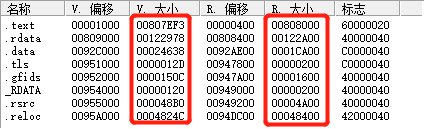
\includegraphics[width=10cm]{jie.png}
	\bicaption{Aseprite加壳前节表}{Aseprite Packing Front Section Table}
	\label{jie}
\end{figure}
\begin{figure}[htbp]
	\centering
	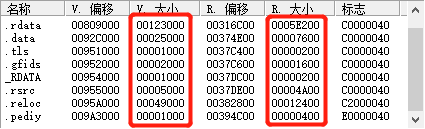
\includegraphics[width=10cm]{jiehou.png}
	\bicaption{Aseprite加壳后节表}{Aseprite packed back section table}
	\label{jiehou}
\end{figure}


通过对图\ref{jie}和图\ref{jiehou}中的红色框出数据分析,在加壳后,PE文件中的节表数据已经被修改, 并且添加了加壳用到的新节.pediy,此时大部分节表数据已经被压缩,成功添加了.pediy新节。
aseprite程序加壳后的运行时情况成功打开,与加壳功能一致,表明加壳成功。运行结果一致,加壳后的程序能够正常运行,表明加密壳的功能正常,能够对PE文件的有效加壳。


\subsection{二进制混淆器功能验证}

二进制混淆器只有一个可执行文件shell.exe,对文件Calculator.exe进行混淆,Calculator为Windows10中自带的计算器,下面通过查看Calculator.exe程序在混淆前后的函数间的调用变化在说明保护的有效性。使用二进制混淆器对Calculator加密后的运行情况如图\ref{jisuanqi}所示。

\begin{figure}[htbp]
	\centering
	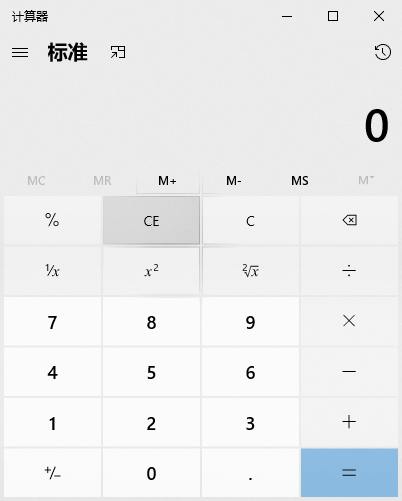
\includegraphics[width=6cm]{jisuanqi.png}
	\bicaption{Calculator.exe使用二进制混淆后的运行情况}{Operation of Calculator.exe after using binary obfuscation}
	\label{jisuanqi}
\end{figure}

计算器的功能正常运行,为了更深入的测试二进制混淆效果,下面使用IDA PRO对该程序进行反汇编,通过查看Calculator程序在混淆前后的函数控制流来观察加密的有效性。在加密前后Calculator的函数sub\_403339的控制流图分别如图\ref{403339}和图\ref{403339}所示,图中序号表示函数内部的基本块序号。
\begin{figure}[htbp]
	\centering
	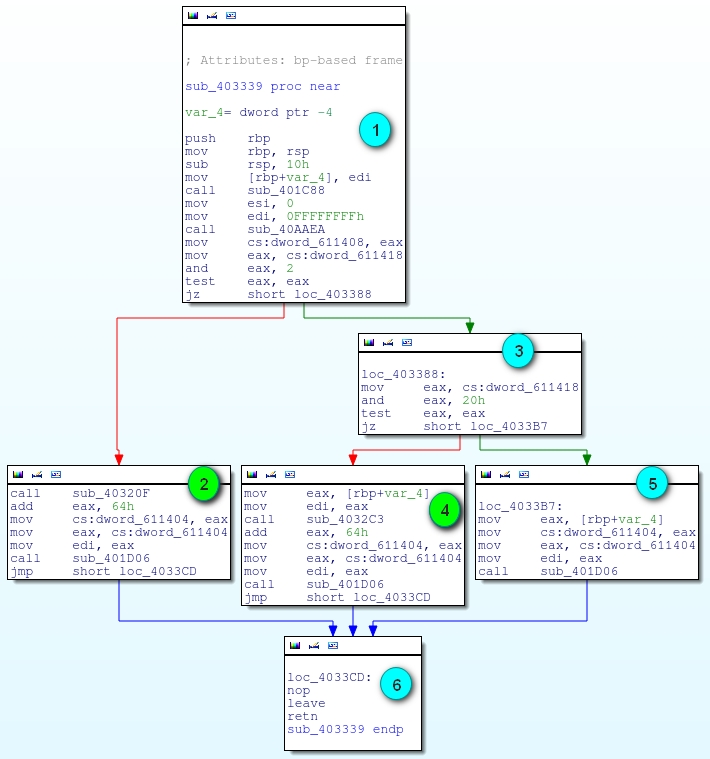
\includegraphics[width=14cm]{403339.jpg}
	\bicaption{加密前sub\_403339函数的控制流图IDA截图}{Control flow diagram of sub\_403339 function before encryption}
	\label{403339}
\end{figure}
\begin{figure}[htbp]
	\centering
	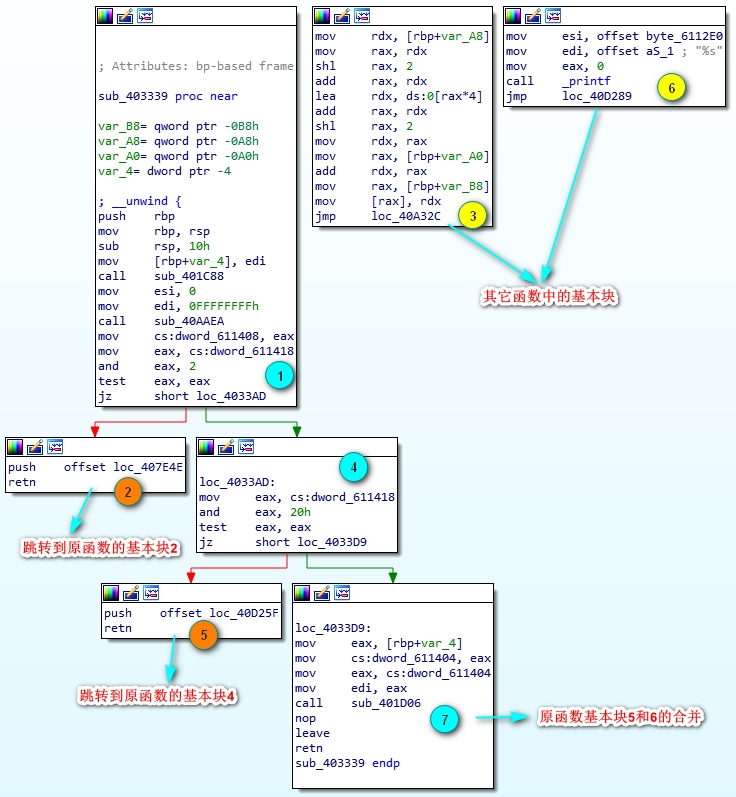
\includegraphics[width=14cm]{403339hou.jpg}
	\bicaption{加密后sub\_403339函数的控制流图IDA截图}{Control flow diagram of sub\_403339 function after encryption}
	\label{403339hou}
\end{figure}

由图\ref{403339}和图\ref{403339hou}可知,加密前后函数sub\_403339分别包含了6个和7个基本块。加密后,原函数的1和3基本块加密前后基本没有发生变化,分别对应加密后的1和4基本块;原函数中5和6基本块内容也没有变化,加密后被合成了基本块7;原函数中的2和4基本块被交换到了其他函数中;加密后函数中多了两个其他函数的3和6基本块,且基本块最后是一条jmp指令,通过该jmp指令将控制流转移到下一个基本块;原函数中对于基本块2和4的控制流转移通过基本块2和5中push+retn型指令实现。

加密后,参与加密函数内部的部分基本块被交换到了其他函数中,被交换的基本块通常有其他的函数的基本块,加大了使用IDA等静态分析器的分析难度,整个程序的控制流信息被打乱。

综上可知,二进制混淆器对程序进行加密后,原有的控制流信息得到了隐藏,达到了对PE文件加密的目的,二进制混淆器功能正常。

\section{性能评估}

性能评估在32位Windows10系统下,内存为2G,磁盘空间为60G下进行,评估内容包括静态混淆技术加密保护和虚拟机保护有效性。使用的测试样本为Windwos10下自带程序和目前流行软件。

\subsection{虚拟机加壳性能评估}

本节将对虚拟机加壳与流行加壳软件进行性能对比,其中包括压缩壳和加密壳,对比的变量为不同的测试程序,对比的输出数据为程序加壳后的大小、开启用时、和执行一次任务所用时间对比,通过计算得出压缩率、启动时间延迟百分比,额外运行时间开销百分比。

使用UPX软件这款压缩壳作为对照组。这里说明一下,使用UPX压缩壳软件作为对照组,是因为软件虚拟机加壳下,使用虚拟机加壳,相当于软件内置一个虚拟机解释器,在执行过程中采用边执行二进制代码边进行解释,程序的运行时间是最重要的性能指标,所以,在能保证程序正常运行的情况下,程序的运行时间是最重要的参考指标。至于加密壳,其运行时间远远小于虚拟机加壳,在这一方便,虚拟机加壳性能与加密壳性能差距太大, 所以不能作为对照组。尽管UPX是一个压缩壳,但是现在未公布的Windows压缩壳大部分是参考UPX进行修改,所以使用UPX作为加壳对照组具有一定意义。

% Please add the following required packages to your document preamble:
% \usepackage{multirow}
% Please add the following required packages to your document preamble:
% \usepackage{multirow}
\begin{table}[htbp]
	\centering
	\bicaption{测试程序加壳前后大小变化}{The size change of the test program before and after packing}
	\begin{tabular}{c|c|cc|cc}
		\bottomrule[1.5pt]
		\multirow{2}{*}{测试程序} & 原始程序   & \multicolumn{2}{c|}{UPX加壳后} & \multicolumn{2}{c}{加密壳加壳后} \\ \cline{2-6} 
		& 大小(KB) & 大小(KB)       & 压缩率(\%)      & 大小(KB)     & 额外空间开销(\%)     \\ \hline
		maps                  & 21     & 8            & 40.9         & 40         & 93.0           \\ \hline
		cacls                 & 33     & 8            & 26.9         & 45         & 38.7           \\ \hline
		mkdir                 & 72     & 32           & 45.7         & 110        & 54.0           \\ \hline
		bscmake               & 95     & 36           & 37.9         & 116        & 23.0           \\ \hline
		ls                    & 146    & 35           & 24.5         & 156        & 7.6            \\ \hline
		aseprite              & 3668   & 656          & 17.9         & 3851       & 0.5            \\ 
		\toprule[1.5pt]
	\end{tabular}

	\label{changesize}
\end{table}


从表\ref{changesize}可以看出,在测试程序大小小于100KB时,加壳导致的额外空间开销明显降低了,程序aseprite加壳后产生的额外空间开销甚至只有0.5$\%$。

% Please add the following required packages to your document preamble:
% \usepackage{multirow}
\begin{table}[htbp]
	\centering
			
	\bicaption{测试程序加壳前后时间变化}{Time changes before and after the test program is packed}
	\begin{tabular}{l|l|ll|ll}
		\bottomrule[1.5pt]
		\multirow{2}{*}{测试程序} & 原始程序 & \multicolumn{2}{l|}{UPX加壳后} & \multicolumn{2}{l}{加密壳加壳后} \\ \cline{2-6} 
		&
		\begin{tabular}[c]{@{}l@{}}平均运行\\ 时间(ms)\end{tabular} &
		\begin{tabular}[c]{@{}l@{}}平均运行\\ 时间(ms)\end{tabular} &
		\begin{tabular}[c]{@{}l@{}}额外时间\\ 开销(\%)\end{tabular} &
		\begin{tabular}[c]{@{}l@{}}平均运行\\ 时间(ms)\end{tabular} &
		\begin{tabular}[c]{@{}l@{}}额外时间\\ 开销(\%)\end{tabular} \\ \hline
		maps                  & 5    & 8           & 66.7\%        & 6            & 33.3         \\ \hline
		
		cacls                 & 120  & 127         & 6.2           & 131          & 9.8          \\ \hline
		mkdir                 & 44   & 47          & 8.1           & 51           & 16.3         \\ \hline
		bscmake               & 253  & 272         & 7.6           & 275          & 9.0          \\ \hline
		ls                    & 30   & 31          & 4.9           & 32           & 8.5          \\ \hline
		aseprite              & 540  & 561         & 3.9           & 564          & 4.5          \\
	    \toprule[1.5pt]
	\end{tabular}

	\label{changetime}
\end{table}
从表\ref{changetime}可以看出,使用本文加密壳加壳后的程序额外运行时间比较少,和UPX加壳软件加壳后产生的额外运行时间开销接近。时间开销相对不大的一个原因是加密壳只进行了函数间基本块的交换,使用随机算法,没有对程序汇编代码进行压缩,时间复杂度较低,如果需要对加密性能进行强化,可以使用更复杂或使用自定义的加密算法。所以,加密壳加壳后程序产生的额外时间和空间开销比较小,可以较好地满足实际应用。


\subsection{二进制混淆器功能评估}

本节通过二进制混淆器的指令执行效率进行评估来判断本文提出的混淆算法的有效性,评估的指标包括程序混淆后的混淆强度、运行时间开销、稳定性、隐蔽性。

为对比系统中混淆器的性能情况,使用市面上流行的二进制代码混淆工具Virbox Protector对程序混淆后的结果作为对照。

\subsubsection{混淆强度}

混淆强度的评估使用赵玉洁等提出的控制流循环复杂度和单条指令执行效率来度量。其中指令执行效率的公式为:$\mathit{IE = Id/Is}$,其中$\mathit{Is}$、$\mathit{Id}$分别表示被测试程序所包含的总指令数量和被测试程序中被运行过的指令数量;控制流循环复杂度的公式为:$\mathit{V(G)=e-n+2}$,其中e表示边的总数,n表示节点(基本块)的总数,测试程序经过混淆器混淆前后的指令执行率如表\ref{order}所示。

% Please add the following required packages to your document preamble:
% \usepackage{multirow}
\begin{table}[htbp]
	\centering
	\bicaption{混淆器混淆前后测试程序的指令执行率}{The instruction execution rate of the test program before and after obfuscation}
	\begin{tabular}{c|ccc|ccc}
		\bottomrule[1.5pt]
		\multirow{2}{*}{测试程序} & \multicolumn{3}{c|}{原始程序} & \multicolumn{3}{c}{混淆后程序} \\ \cline{2-7} 
		&
		\begin{tabular}[c]{@{}c@{}}静态指令\\ 数(条)\end{tabular} &
		\begin{tabular}[c]{@{}c@{}}动态指令\\ 数(条)\end{tabular} &
		\begin{tabular}[c]{@{}c@{}}执行率\\ (\%)\end{tabular} &
		\begin{tabular}[c]{@{}c@{}}静态指令\\ 数(条)\end{tabular} &
		\begin{tabular}[c]{@{}c@{}}动态指令\\ 数(条)\end{tabular} &
		\begin{tabular}[c]{@{}c@{}}执行率\\ (\%)\end{tabular} \\ \hline
		maps                  & 4755    & 1059   & 22.27  & 4899     & 1210   & 24.69  \\ \hline
		cacls                 & 3306    & 761    & 23.01  & 3514     & 810    & 23.05  \\ \hline
		mkdir                 & 21230   & 4097   & 19.29  & 22019    & 4600   & 20.89  \\ \hline
		bscmake               & 8185    & 1975   & 24.12  & 9100     & 2216   & 24.35  \\ \hline
		ls                    & 12523   & 2439   & 19.47  & 12699    & 3010   & 23.70  \\ \hline
		aseprite              & 193966  & 32374  & 16.68  & 196109   & 41409  & 21.11  \\
		\toprule[1.5pt]
	\end{tabular}

	\label{order}
\end{table}
程序在混淆之后,静态指令和动态指令都有所增加,这是因为采用了建立索引进行函数间基本块交换的混淆算法,在原有程序的基础上,增加了一些指令数据来实现函数间的跳转,虽然跳转的只是一些MOV、ADD、SUB等不影响寄存器和堆栈的指令,但是其指令数量还是有所提高,由原始程序和混淆程序的指令执行率可知,程序中每条执行被执行概率增加了,一定程序上反映出了程序的复杂性增加了。使用Virbox Protector混淆后程序的执行执行效率如表\ref{Virbox}。

\begin{table}[htbp]
	\centering
	\bicaption{Virbox Protector混淆后程序的指令执行率}{The instruction execution rate of the program after Virbox Protector confusion}
	\begin{tabular}{cccccc}
		\bottomrule[1.5pt]
		测试程序     & Ftotal & Fobf & 静态指令数  & 动态指令数 & 指令执行率 \\ \hline
		maps     & 126    & 14   & 4518   & 1198  & 26.51 \\
		cacls    & 39     & 7    & 3214   & 943   & 29.34 \\
		mkdir    & 234    & 15   & 14981  & 4709  & 31.43 \\
		bscmake  & 157    & 15   & 4910   & 1598  & 32.54 \\
		ls       & 164    & 14   & 46910  & 6102  & 13.00 \\
		aseprite & 6019   & 99   & 259838 & 34631 & 13.32 \\ 
		\toprule[1.5pt]
	\end{tabular}

	\label{Virbox}
\end{table}
其中FOBF、FTOTAL分别表示参与混淆的函数个数和程序的函数总数。从表\ref{Virbox} 可以看出几点:1.经过Virbox Protector混淆之后,不同程序的静态执行数量出现了增加和减少两种情况,这是Virbox Protector的混淆机制导致的,使用IDA Pro查看混淆后的程序的二进制汇编代码可知,在反汇编之后存在大量的数据,在静态反汇编时是以db指令存在的,被反汇编当做数据对待,但在执行时,其实在被解密后是以普通汇编指令执行的;2.当程序增加较多的静态指令数量时,程序的指令执行率未混淆之前甚至高于混淆之后,当增加较少的静态指令数量时,程序的执行效率比混淆前要高很多。所测试的程序指令执行率有减少也有增加,这是因为Virbox Protector内部使用了不同的混淆机制,本课题只使用一种,比如某些垃圾指令不被执行会降低程序的指令执行效率,而将一条会被执行的指令拆分成多条执行或添加被执行的垃圾执行会提高程序执行率。

测试程序在混淆前后控制流循环复杂度如表\ref{protector_2}所示。

\begin{table}[htbp]
	\centering
	\bicaption{混淆前后测试程序控制流循环复杂度}{Test program control flow loop complexity before and after confusion}
	\begin{tabular}{c|c|cc|cc}
		\bottomrule[1.5pt]
		\multirow{2}{*}{测试程序} & \multirow{2}{*}{原始复杂度} & \multicolumn{2}{c|}{Virbox Protector混淆后} & \multicolumn{2}{c}{混淆器混淆后} \\ \cline{3-6} 
		&       & 复杂度   & 增长率(\%) & 复杂度   & 增长率(\%) \\ \hline
		maps     & 267   & 184   & -31.1   & 279   & 4.49    \\
		cacls    & 318   & 123   & -61.3   & 329   & 3.45    \\
		mkdir    & 778   & 1690  & 117.2   & 920   & 18.25   \\
		bscmake  & 378   & 298   & -21.2   & 451   & 19.31   \\
		ls       & 934   & 3890  & 316.4   & 1090  & 16.70   \\
		aseprite & 34509 & 40109 & 16.2    & 37909 & 9.85    \\ 
		\toprule[1.5pt]
	\end{tabular}

	\label{protector_2}
\end{table}

使用Virbox Protector混淆后的程序的的控制流循环复杂度没有固定的规则,控制流循环复杂度有的数据特别高,有的甚至出现负数。而经过本课题的混淆器混淆之后,基本控制流的复杂度和增长率可以呈现一定的规律,程序的增长率基本维持在7$\%$-11$\%$,这说明在不考虑垃圾指令优化时,使用单种混淆方式通常情况下复杂度是增加的。

值得注意的是,Virbox Protector处理过后的程序的控制流循环复杂度降低了,但是并不代表程序的控制减少了,由于Virbox Protector包含多种混淆机制,在执行时有大量的数据需要解密后执行,所以程序的动态控制流会更复杂。

根据上述测试结果,可以得到二进制混淆器加密前后指令复杂性和控制流循环复杂度的变化以及与Virbox Protector软件的混淆结果对比,可以看到,经过二进制混淆器混淆后的程序的指令复杂度得到一定提高,表明混淆算法的混淆强度指标合格。同时也反映出了通过指令的执行率和控制流循环夫再度来衡量代码混淆程序的局限性。

\subsubsection{运行时间开销的对比}


二进制混淆器和Virbox Protector对测试程序混淆后,程序的运行时间开销的对比如表\ref{shijianhunxiao}


\begin{table}[htbp]
	\centering
	\bicaption{混淆后测试程序的额外开销}{Additional overhead of test program after obfuscation}
	\begin{tabular}{c|cc|cccc}
		\bottomrule[1.5pt]
		\multirow{2}{*}{测试程序} & \multicolumn{2}{c|}{原始程序} & \multicolumn{2}{c}{混淆器混淆后}      & \multicolumn{2}{c}{额外开销} \\ \cline{2-7} 
		&
		大小(KB) &
		\begin{tabular}[c]{@{}c@{}}平均运行\\ 时间(ms)\end{tabular} &
		大小(KB) &
		\multicolumn{1}{c|}{\begin{tabular}[c]{@{}c@{}}平均运行\\ 时间(ms)\end{tabular}} &
		\begin{tabular}[c]{@{}c@{}}空间\\ (\%)\end{tabular} &
		\begin{tabular}[c]{@{}c@{}}时间\\ (\%)\end{tabular} \\ \hline
		maps                  & 40           & 3          & 43   & \multicolumn{1}{c|}{5}   & 7.5         & 66.7       \\ \hline
		cacls                 & 78           & 157        & 85   & \multicolumn{1}{c|}{170} & 8.9         & 8.2        \\ \hline
		mkdir                 & 124          & 223        & 130  & \multicolumn{1}{c|}{131} & 5.6         & 5.6        \\ \hline
		bscmake               & 68           & 28         & 72   & \multicolumn{1}{c|}{32}  & 5.8         & 14.2       \\ \hline
		ls                    & 120          & 91         & 128  & \multicolumn{1}{c|}{101} & 6.7         & 10.9       \\ \hline
		aseprite              & 5093         & 450        & 5609 & \multicolumn{1}{c|}{480} & 10.1        & 6.7        \\ 
		\toprule[1.5pt]
	\end{tabular}

 	\label{shijianhunxiao}
\end{table}

使用二进制混淆器后,程序的额外占用空间随着程序的占用空间增大而增大,空间开销在程序小于5M时空间开销低于10$\%$;程序的额外运行时间开销随着运行时间增加比例大约在8$\%$左右。由以上可得,二进制混淆器产生的额外开销所占比率并不高。由表\ref{ewaikaixiao}可知,

\begin{table}[htbp]
	\centering
	\bicaption{Virbox Protector混淆后测试程序的额外开销}{The extra cost of the test program after Virbox Protector obfuscation}
	\begin{tabular}{ccccc}
		\bottomrule[1.5pt]
		测试程序     & 大小(KB) & 空间开销(倍) & 时间(ms) & 时间开销(倍) \\ \hline
		maps     & 484    & 11.0    & 10.3   & 3.44    \\
		cacls    & 1723.8 & 22.1    & 282.6  & 1.8     \\
		mkdir    & 1277.2 & 10.3    & 691.3  & 3.10    \\
		bscmake  & 632.4  & 9.3     & 81.4   & 2.91    \\
		ls       & 588    & 4.9     & 171.9  & 1.89    \\
		aseprite & 6111.6 & 1.2     & 49.5   & 1.10    \\ 
		\toprule[1.5pt]
	\end{tabular}

	\label{ewaikaixiao}
\end{table}

使用Virbox Protector混淆后的程序的占用空间和运行时间开销都很高,这样会程序在实际使用起来的体验不如本课题的二进制混淆器。

\subsubsection{隐蔽性}

本课题隐蔽性通过计算经过二进制混淆前后的文件相似度来判断。 测试样本的混淆前后文件相似度使用radare中的radiff2工具来计算,经过混淆前后的相似度如表\ref{protector_2}所示。使用Virbox Protector加密过的程序的变化非常明显,可以很明确看出程序是经过混淆处理的,这样的程序隐蔽性较低。


\begin{table}[htbp]
	\centering
	\bicaption{混淆前后程序的相似度}{Program similarity before and after confusion}

	\begin{tabular}{c|c|c|c|c|c|c}
		\bottomrule[1.5pt]
		测试程序      & maps & cacls & mkdir & bscmake & ls & aseprite \\ \hline
		相似度(\%)   & 91   & 93    & 95    & 92      & 93 & 92       \\ \hline
		平均相似度(\%) & \multicolumn{6}{c}{93}                        \\ 
		\toprule[1.5pt]
	\end{tabular}
	\label{xiangsidu}
\end{table}

由表\ref{xiangsidu}可知,混淆前后,程序的相似度比较高,都在80$\%$以上,平均相似度为89$\%$。从上面可以得出,使用本课题的虚拟机的混淆程序不易被发现该程序是经过混淆的,这样降低了程序被逆向的风险,所以具有一定的抗逆向意义。

二进制混淆器与Virbox Protector对比,本文设计的二进制混淆器的混淆强度较低,同时在被逆向的情况下,本课题的保护壳更容易被成功逆向破解,这是因为本混淆器只实现了普通汇编指令如MOV、SUB、ADD等不影响寄存器和堆栈空间的指令的交换和混淆,如果将所有汇编指令都实现交换和混淆,产生的二进制混淆器的混淆强度将会高出一个级别。但是本文的二进制混淆器的运行时间、占用磁盘空间和隐蔽性能比较良好。

综上可知,加密后的程序的运行时间、磁盘占用空间和隐蔽性都要优于Virbox Protector,具有较好的实用性。这表明本文二进制混淆器的抵抗静态分析的能力较强,但是抵御动态分析方面存在不足。由上文可知,本混淆器可以与其他加壳工具兼容,实现混用,本文的二进制混淆器与其他保护壳共同使用时,可以产生较高的保护力。由此表明本文所提出的二进制混淆算法可以提高软件的抗逆向性能。

\section{本章小结}

本章首先对系统的实现和所选择的测试环境进行介绍,然后分别对虚拟机加壳器和二进制混淆器的功能进行了验证和性能进行评估,由实验结果可知,加壳器和二进制混淆器的功能正常、性能评估结果表明使用上述保护方法对二进制可执行程序进行保护具有一定实用性,总体实验结果表明所提出的虚拟机加壳方法和二进制混淆器组成的保护系统能够有效增强Windows下可执行程序的抗逆向能力。




















\begin{conclusion}

恶意的逆向分析技术严重威胁着软件的版权安全,本文针对Windows平台下x86架构下的可执行文件进行了软件保护技术方面的探索,提出了一种基于虚拟机加壳的多样化Handler动态保护方法和一种建立索引的方式对函数间基本块进行交换的静态保护算法。本文从代码层面上对算法进行了阐述,描述了软件保护机制的实现方法,给出了虚拟机加壳技术和静态二进制混淆技术的核心汇编源码,并对设计的核心数据结构进行了说明,本论文的工作总结如下:

首先,PE 文件加壳技术的研究。首先对 PE 文件的加载过程和 PE 文件的文 件结构进行分析,在虚拟机加壳的基础上,提出了多样 化 Handler 虚拟机加壳技术,对同一个 Handler 进行多样化的指令实现,使得同一个功能模块有不同的二进制指令实现,有效了增加逆向分析者的分析成本。 

其次,PE 二进制混淆技术的研究。首先对二进制混淆技术进行了分析,总结 常见二进制混淆方法的不足,提出了建立索引进行函数间基本块交换的混淆算 法,提出了对 PE 文件进行基本块交换后的重构 方法。

最后,根据提出的 虚拟机加壳技术和二进制混淆算法设计并实现了一个PE 文件保护系统,系统包括 PE 文件虚拟机加密壳和 PE 文件二进制混淆器。对该系 统的设计与实现进行了详细阐述,并对 PE 文件虚拟机加密壳和 PE 文件二进 制混淆器进行了功能的验证和性能评估。实验结果表明提出的多样化 Handler 虚 拟机加壳方式和二进制代码混淆算法均有效,有效增强了 Windows 的 PE 文 件的抗逆向分析能力。


  
\end{conclusion}


% \begin{table}[H]
%   \bicaption{中文}{english}
%   \aboverulesep=0ex
%   \belowrulesep=0ex
%   \begin{tabularx}{\columnwidth}{@{} C|C @{}}
%       \toprule[1.5pt]
%       Key                 & Value    \\
%       \hline
%       simulation duration & 12 hours \\
%       \hline
%       update interval     & 1s       \\
%       \hline
%       time-to-live        & 12 hours \\
%       \hline
%       buffer size         & infinite \\
%       \hline
%       message interval    & 20s      \\
%       \bottomrule[1.5pt]
%   \end{tabularx}
%   \label{table: simulation parameters}
% \end{table}
%%% 其它部分
%% 参考文献
% 注意:至少需要引用一篇参考文献,否则下面两行可能引起编译错误。
% 如果不需要参考文献,请将下面两行删除或注释掉。
\bibliographystyle{thuthesis-numeric}      % 顺序编码制
% \bibliographystyle{thuthesis-author-year}  % 著者-出版年制
% \bibliographystyle{thuthesis-bachelor}     % 本科生参考文献的著录格式
\bibliography{ref/refs}
%% 个人简历
\begin{resume}

%  \researchitem{研究成果} % 有就写,没有就删除
  \begin{achievements}
    \item 哈尔滨理工大学. Windows下可执行文件压缩加密程序软件 V1.0: 中国,(软件著作权登记号为2020SR1581640) . 
  \end{achievements}

\end{resume}


%% 致谢
\begin{acknowledgement}
本人软件保护工程方面做了些微小的工作,仅仅围绕了抗逆向技术做了边缘性的优化工作,并没有做其技术的核心优化。不过从没有太多参考的当下从0到1建立了一个完整系统,且结果也恰好说明这个系统确实有效,也是一件颇为有趣的事情。当然这里少不了我的家人、老师和朋友们的功劳。

首先致谢我的父母,支持我完成本科教育后继续学习,使得我满足自己的好奇和求知欲。其次感谢我的导师李老师,接触的四年里共同奋斗过很多事情,有欢乐也有忧愁,所有教导我都铭记于心,并且在毕业设计之际允许我完成自己的想法。接着感谢我的朋友们,在我的毕业设计之际提供了无数关怀与帮助,使我完成之。最后感谢在哈尔滨这个城市直接或间接教导我的所有人,谢谢。

最后,再次一并感谢。
    
  
\end{acknowledgement}





%% 本科生要这几个索引,研究生不要。选择性留下。
% 插图索引
%\listoffigures
% 表格索引
%\listoftables
% 公式索引
%\listofequations

%% 附录
%\begin{appendix}
%\chapter{传感器的标定}
\label{cha:calibrations}

\subsection{相机的标定}
\label{cam_calib}
视觉传感器因感光元件有异而分为CMOS相机和CCD相机,由于CMOS受其成像原理所限,无法像CCD相机那样同时接收并处理所有光信号,即卷帘快门产生的“果冻”现象\cite{solutions2011shutter}。但全局快门CMOS相机通过为每个像素点增加了采样保持单元,使其可以同时接收并处理所有光信号,消除了“果冻”效应,可以更好地保留瞬态成像的原本面貌。而相机由于在生产的过程中,不同批次和工艺都会产生一定的差异,故在实际使用之前需要对其进行标定。标定是通过一系列标准的办法估计出相机的一些关键指标参数、外部参数和畸变参数。关键指标参数即所谓的相机内部参数,包括相机的焦距、像元大小和光学中心坐标;外部参数是因为相机的自身转动和平移产生的变化;而畸变参数是由于透镜的存在产生的。

在相机的标定上,卷帘快门和全局快门的相机二者要区分对待。由于卷帘快门因其在移动成像过程中会发生畸变,对其标定需要根据传感器的电子快门时间进行精确的建模,而后对畸变进行矫正。

卷帘快门的标定实际上是对其线延迟进行计算,并尽可能地使计算结果逼近它的真实值。如Luc Oth等人的方法\cite{oth2013rolling},是从一般的投影方程出发,提出了一个适用于卷帘快门相机的连续时间透视投影模型,并给出了相关的透视定位理论。在推导了线延迟估计方程之后,将其与透视姿态方程相结合,基于一组已知的标志点同时估计摄像机姿态和线延迟。最后,通过推导重投影误差的协方差矩阵,建立了标准的最大似然估计量。由于实际SLAM应用中较少考虑使用卷帘快门相机,故不在此详述方法。

而对于全局快门相机,则无需考虑上述内容,直接进行相机的参数标定。

一般,我们使用针孔模型为单个相机的数学模型,如\ref{cha2:equ:cam0}所示。本节所述的所有内容均建立在相机的参考坐标系中。

\begin{equation}
  \label{cha2:equ:cam0}
  s\begin{bmatrix}
    u\\
    v\\
    1
  \end{bmatrix}
  = \mathbf{A}[\mathbf{R}|\mathbf{t}]\mathbf{M}'
\end{equation}

其中

\begin{equation}
  \mathbf{A} = \begin{bmatrix}
    f_x & 0   & c_x\\
    0   & f_y & c_y\\
    0   & 0   & 1
  \end{bmatrix},\ 
  [\mathbf{R}|\mathbf{t}] = \begin{bmatrix}
    r11 & r12 & r13 & t1\\
    r21 & r22 & r23 & t2\\
    r31 & r32 & r33 & t3
  \end{bmatrix},\ 
  \mathbf{M}' = \begin{bmatrix}
    X\\
    Y\\
    Z\\
    1
  \end{bmatrix}
\end{equation}

$\mathbf{A}$矩阵是相机的内部参数矩阵,其中$f$代表焦距,$c$代表光心;$[\mathbf{R}|\mathbf{t}]$是相机在世界坐标系下的旋转和平移矩阵,也被称为相机的外部参数矩阵;$\mathbf{M}'$是图像中的点在世界参考系下对应的三维坐标。由于成像的过程是将三维坐标中的点投影在二维平面上,这个过程丢失了深度维度,也对投影的像进行了尺度化转换,即将真实坐标点转化为像的二维坐标点。

\begin{equation}
  \label{cha2:eqa:xy2uv}
  \begin{aligned}
    &u = f_x * x' + c_x\\
    &v = f_y * y' + c_y
  \end{aligned}  
\end{equation}

其中

\begin{equation}
  \begin{cases}
    x' = \frac {x} {z}\\
    y' = \frac {y} {z}
  \end{cases},\ \begin{bmatrix}
    x\\
    y\\
    z
  \end{bmatrix} = \mathbf{R}\begin{bmatrix}
    X\\
    Y\\
    Z
  \end{bmatrix} + \mathbf{t}
\end{equation}

但实际情况下,由于直接使用针孔相机会导致进光量的急剧减少,故常常我们使用透镜代替针孔的位置,但这一方法引入了畸变,也常被称为失真。透镜畸变从效果上分为两种,分别是桶形畸变和枕形畸变,如图所示。在桶形失真中,图像放大倍率随其像素位置与光轴的距离而减小。明显的效果是在球体(或桶)周围映射的图像的效果。鱼眼镜头采用半球形视图,利用这种畸变将无限宽的物平面映射到有限的图像区域。在变焦镜头镜筒中,畸变出现在镜头焦距范围的中间,在该范围的广角端最严重。枕形畸变则相反,在枕形畸变中,图像放大率随其像素位置与光轴的距离而增加。可见的效果是,未穿过图像中心的线像枕形一样向内弯曲,朝向图像中心。综合两种畸变的效果还会产生一种畸变,我们称之为胡子形畸变。其名字由于其特殊的畸变形态而来,在偏向中心的位置,其畸变于桶形畸变相似,而向外的位置却又与枕形畸变相似。

但是,无论是哪种畸变,一般都可以利用公式\ref{equ:chap2:distortion01}和公式\ref{equ:chap2:distortion02}共同表示。

\begin{equation}
\label{equ:chap2:distortion01}
\begin{aligned}
x'' = x_d &+ (x_d - x_c)(k_1r^2 + k_2r^4 \dots)\\&+(p_1(r^2 + 2(x_d - x_c)^2)\\&+ 2p_2(x_d - x_c)(y_d - y_c))(1 + p_3r^2 + p_4r^4 \dots)
\end{aligned}
\end{equation}
\begin{equation}
\label{equ:chap2:distortion02}
\begin{aligned}
y'' = x_d &+ (x_d - x_c)(k_1r^2 + K_2r^4 + \dots)\\&+(2p_1(x_d - x_c)(y_d - y_c) \\&+ p_2(r^2 + 2(y_d - y_c)^2))(1 + p_3r^2 + p_4r^4 \dots)
\end{aligned}
\end{equation}

在公式\ref{equ:chap2:distortion01}和公式\ref{equ:chap2:distortion02}中,$x_d$和$y_d$分别是镜头在x和y方向的像平面投影的畸变像点,$x_u$和$y_u$是理想针孔相机投射出的未畸变的像点,$x_c$和$y_c$是光心,$k_n$和$p_n$分别是在径向和切向的$n$阶畸变系数,而$r$是$\sqrt{(x_d - x_c)^2 + (y_d - y_c)^2}$。将x$x''$和$y''$分别带入公式\ref{cha2:eqa:xy2uv}中并替换$x'$和$y'$,便可将畸变参数加入模型中。

\begin{equation}
\label{cha2:equ:cam1}
  \begin{aligned}
    &u = f_x * x'' + c_x\\
    &v = f_y * x'' + c_y
  \end{aligned}
\end{equation}

此外,由于某些使用场景的原因,相机的图像传感器可能是由于需要聚焦于斜面而倾斜,这会导致$x$和$y$的透视变形,这种变形可以通过\ref{cha2:equ:cam2}的模型来表示。

\begin{equation}
\label{cha2:equ:cam2}
  s\begin{bmatrix}
    x'''\\
    y'''\\
    1
  \end{bmatrix} = \begin{bmatrix}
    \mathbf{R}_{33}(\tau_x,\tau_y) & 0 & -\mathbf{R}_{13}(\tau_x,\tau_y)\\
    0 & \mathbf{R}_{33}(\tau_x,\tau_y) & -\mathbf{R}_{23}(\tau_x,\tau_y)\\
    0 & 0 & 1
  \end{bmatrix} \mathbf{R}(\tau_x,\tau_y)\begin{bmatrix}
    x''\\
    y''\\
    1
  \end{bmatrix}
\end{equation}

其中,$\tau_x$和$\tau_y$分别是两个方向的角度参数,而$\mathbf{R}(\tau_x,\tau_y)$如\ref{cha2:equ:cam3}所示。

\begin{equation}
\label{cha2:equ:cam3}
\begin{aligned}
  \mathbf{R}(\tau_x,\tau_y) &= \begin{bmatrix}
    \cos(\tau_y) & 0 & -\sin(\tau_y)\\
    0 & 1 & 1\\
    \sin(\tau_y) & 0 & \cos(\tau_y)
  \end{bmatrix}\begin{bmatrix}
    1 & 0 & 0\\
    0 & \cos(\tau_x) & \sin(\tau_x)\\
    0 & -\sin(\tau_x) & \cos(\tau_x)
  \end{bmatrix}\\ &= \begin{bmatrix}
    \cos(\tau_y) & \sin(\tau_y)\sin(\tau_x) & -\sin(\tau_y)\cos(\tau_x)\\
    0 & \cos(\tau_x) & \sin(\tau_x)\\
    \sin(\tau_y) & -\cos(\tau_y)\sin(\tau_x) & \cos(\tau_y)\cos(\tau_x)
  \end{bmatrix} 
\end{aligned}
\end{equation}

最后,需将\ref{cha2:equ:cam1}中的$x''$和$y''$替换为\ref{cha2:equ:cam2}中的$x'''$和$y'''$,如\ref{cha2:equ:cam4}所示。

\begin{equation}
\label{cha2:equ:cam4}
\begin{aligned}
  &u = f_x * x''' + c_x\\
  &v = f_y * y''' + c_y
\end{aligned}
\end{equation}

至此,所有需要通过标定获得的相机参数已定,如\ref{cha2:equ:campara}所示,$k$值的数量一般根据相机透镜的畸变程度而定,如畸变较大的相机可取值到6个,而普通相机的取值数量一般是2到4个。

\begin{equation}
\label{cha2:equ:campara}
  (f_x,f_y,c_x,c_y,k_1,k_2,p_1,p_2,k3,k4,k5,k6,s1,s2,s3,s4,\tau_x,\tau_y)
\end{equation}

一般我们使用标定板辅助相机的参数标定,为了保证标定效果,需要尽可能地让相机成像的所有位置都拍摄过标定板。标定板按照图案可分为棋盘板、方块板、正六边形板和圆点板,需要注意的是,标定板的不同会产生不同的标定结果,但相互之间误差不会大到影响对相机的使用和计算。大多数正常使用的情况,如果不对相机本体造成破坏性的打击或剧烈地冲击,这些相机的参数不会随之发生改变。

经过上述标定后,相机发布的数据才可以被正式使用,数据格式为YUV/MJPEG,帧率和分辨率等依实际传感器及其ISP性能为准。

\subsection{IMU的标定}
\label{imu_calib}
不论是在SLAM技术,还是其他机器人学应用的过程中,IMU都是十分关键的传感器。它提供了自身的位姿变化,并可以通过积分计算获取位姿变化轨迹,轨迹和位姿精度与传感器的选型和计算的滤波算法等都有关。一般在机器人上,我们不考虑使用昂贵的光纤陀螺仪或者庞大的机械陀螺仪获取角速度,而是使用微小灵敏的微机电式的陀螺仪、加速度计和电子罗盘。但这类传感器的问题在于误差较大,需要经过较好的标定和滤波才可以使用。IMU的传感器的误差主要有轴偏差、尺度因子、和偏置与噪声\cite{tedaldi2014robust}。其中加速度计和陀螺仪的测量模型可表示为:

\begin{equation}
  \begin{aligned}
    &\mathbf{a}^{B} = \mathbf{T}^{a}\mathbf{K}^{a}(\mathbf{a}^{S}+\mathbf{b}^{a}+\mathbf{\nu}^{a})\\
    &\mathbf{\omega}^{B} = \mathbf{T}^{g}\mathbf{K}^{g}(\mathbf{\omega}^{S}+\mathbf{b}^{g}+\mathbf{\nu}^{g})
  \end{aligned}
\end{equation}

其中,所有的上标$a$代表与加速度计相关的量,所有的上标$g$代表与陀螺仪相关的量;上标$B$表示正交的参考系,上标$S$是非正交的选准系;$T$是表示轴偏差的矩阵,$K$表示的尺度因子,$\mathbf{b} \in \mathbb{R}^3$和$\nu$分别是偏置和白噪声。

对于加速度计的尺度因子可表示为:

\begin{equation}
  \mathbf{K}^{a} = \begin{bmatrix}
    s^{a}_{x} & 0 & 0\\
    0 & s^{a}_{y} & 0\\
    0 & 0 & s^{a}_{z}
  \end{bmatrix}
\end{equation}

对于陀螺仪的尺度因子可表示为:

\begin{equation}
  \mathbf{K}^{g} = \begin{bmatrix}
    s^{g}_{x} & 0 & 0\\
    0 & s^{g}_{y} & 0\\
    0 & 0 & s^{g}_{z}
  \end{bmatrix}
\end{equation}

对于加速度计的轴偏矩阵可表示为:

\begin{equation}
\label{cha2:equ:imu_tbias_a}
\mathbf{T}^{a} = \begin{bmatrix}
    1 & -\alpha_{yz} & \alpha_{zy}\\
    0 & 1 & -\alpha_(zx)\\
    0 & 0 & 1
  \end{bmatrix}
\end{equation}

对于陀螺仪的轴偏矩阵可表示为:

\begin{equation}
  \label{cha2:equ:imu_tbias_g}
  \mathbf{T}^{g} = \begin{bmatrix}
    1 & -\gamma_{yz} & \gamma_{zy}\\
    \gamma_{xz} & 1 & -\gamma_{zx}\\
    -\gamma_{xy} & \gamma_{yx} & 1
  \end{bmatrix}
\end{equation}

式\ref{cha2:equ:imu_tbias_a}和\ref{cha2:equ:imu_tbias_g}中的$\alpha_{ij}$和${\gamma_{ij}}$分别表示从$i$轴到$j$轴加速度计和陀螺仪的旋转量。

建立传感器的误差模型完毕后,我们可以对其进行依次标定。首先应通过对不同标准姿态的IMU进行静止状态的加速度计值和陀螺仪值的数据采集,标准状态指的是IMU的自坐标系X-Y-Z轴任意一轴与世界坐标系的Y轴平行。一般采集会持续几十次,即旋转几十次IMU传感器并重复采集各个姿态时传感器传回的数据,一般次数越多,计算的效果越好。静止通过式\ref{cha2:equ:static}判断。

\begin{equation}
\label{cha2:equ:static}
  \sigma(t_{w}) = \sqrt{[var_{t_{w}}(\mathbf{a}^{t}_{x})]^{2}+var_{t_{w}}(\mathbf{a}^{t}_{y})]^{2}+var_{t_{w}}(\mathbf{a}^{t}_{z})]^{2}}
\end{equation}

其中,$var_{t_{w}}$代表加速度$\mathbf{a}^{t}$在时间段$t_w$内的方差。判断时,只需通过计算$\sigma(t_{w}) - \sigma(T_{init})$即可,大于零则动态,小于等于则为静态。一般$T_{init}$取50。我们忽略白噪声,为加速度计和陀螺仪建立代价函数,分别有式\ref{cha2:equ:costa}和\ref{cha2:equ:costg}。

\begin{equation}
\label{cha2:equ:costa}
\mathbf{L}(\mathbf{\theta} ^{acc}) = \sum^{M}_{k=1}(||\mathbf{g}||^{2}-||h(\mathbf{a}^{S}_{k},\mathbf{\theta}^{acc})||^{2})^{2}
\end{equation}

其中$\mathbf{\theta} ^{acc}$是加速度计的待求解参数,为:

\begin{equation}
  \mathbf{\theta}^{acc}=[\alpha_{yz},\alpha_{zy},\alpha_{zx},s^{a}_{x},s^{a}_{y},s^{a}_{z},b^{a}_{x},b^{a}_{y},b^{a}_{z}]
\end{equation}

对于陀螺仪的代价函数,有:

\begin{equation}
\label{cha2:equ:costg}
\mathbf{L}(\mathbf{\theta} ^{gyro})=\sum^{M}_{k=2}||\mathbf{u}_{a,k}-\mathbf{u}_{g,k}||^{2}
\end{equation}

其中,$\mathbf{\theta} ^{gyro}$是陀螺仪的待求解参数,$\mathbf{u}_{a,k}$是加速度计在旋转后实际测量的重力值,$\mathbf{u}_{g,k}$如\ref{cha2:equ:integ}是通过积分陀螺仪数据之后得到的新的重力向量,它们分别为:

\begin{equation}
  \mathbf{\theta} ^{gyro}=[\gamma_{yz},\gamma_{zy},\gamma_{xz},\gamma_{zx},\gamma_{xy},\gamma_{yx},s^{g}_{x},s^{g}_{y},s^{g}_{z}]
\end{equation}

\begin{equation}
\label{cha2:equ:integ}
\mathbf{u}_{g,k}=\mathbf{\Psi}[w^{S}_{i},\mathbf{u}_{a,k-1}]
\end{equation}

最后,通过Levenberg–Marquardt算法求出参数即可。

而对于电子罗盘的数据标定,则需要在数据融合时进行实时修正。因这种传感器对环境的磁场非常敏感,当处于没有产生较强磁场的物体的环境中,我们通常可以更信赖它的数据,但当周围放置了能够产生较强磁场的物体后,如电机、音响、耳机和麦克风等,电子罗盘的数据会随之产生漂移,这与传感器自身的误差无关,因为环境中的磁场确实受到了干扰发生了改变,而电子罗盘所测得数据也是真实的。所以在工作前校准的结果,是不能保证运行时能够正常工作的。故在建立节点时,我们不对电子罗盘进行校准。

经过上述校准后,IMU发布的数据才可以被使用,数据发布的顺序分别是X-Y-Z轴的加速度,X-Y-Z轴的角速度和X-Y-Z方向的磁力值,更新频率依实际硬件为准。
%\end{appendix}

\end{document}
